%%%%%%%%%%%%%%%%%%%%%%%%%%%%%%%%%%%%%%%%%%%%%%%%%%%%%%%%%%%%%%%%%%%%%%%%%%%%%%%%
%2345678901234567890123456789012345678901234567890123456789012345678901234567890
%        1         2         3         4         5         6         7         8
% DOCUMENT CLASS
\documentclass[a4paper,12pt]{Classes/RoboticsLaTeX}


% USEFUL PACKAGES
% Commonly-used packages are included by default.
% Refer to section "Book - Useful packages" in the class file "Classes/RoboticsLaTeX.cls" for the complete list.
\usepackage{amsmath}
\usepackage{amsfonts}
\usepackage{algorithm}
\usepackage{algorithmic}
\usepackage{multirow}
\usepackage{colortbl}
\usepackage{color}
\usepackage[table]{xcolor}
\usepackage{epigraph}
\usepackage{graphicx}
%\usepackage{subfigure}
\usepackage{caption}
\usepackage{subcaption}
\usepackage{hyperref}
\usepackage{tabularx}
\usepackage{float}
\usepackage{longtable}
\usepackage[pdftex]{graphicx}
\usepackage{pdfpages}
\usepackage{pdflscape}
\usepackage[acronym,toc]{glossaries}
\usepackage{setspace}
\usepackage[utf8]{inputenc}
\usepackage[table]{xcolor}

%\usepackage{layout}

\setstretch{1.5}
%\onehalfspacing


% SPECIAL COMMANDS
% correct bad hyphenation
\hyphenation{op-tical net-works semi-conduc-tor}
\hyphenation{par-ti-cu-lar mo-du-le ge-stu-re}
% INTERLINEA 1.5
%\renewcommand{\baselinestretch}{1.5}

%% ignore slightly overfull and underfull boxes
%\hbadness=10000
%\hfuzz=50pt
% declare commonly used operators
%\DeclareMathOperator*{\argmax}{argmax}

% >>>> Replace all the [[Placeholders]] on the front page and in the Declaration <<<<

\title{\Large{Reinforcement Learning Algorithms for Energy aware VM Selection in Data centre}}

\author{Niju Michael Nicholas}
\collegeordept{School of Computer Science}
\university{University of Galway}
\crest{
\includegraphics[width=140mm]{Figures/University_Of_Galway_Logo__Positive_Landscape.png}}
%\crest{
\includegraphics[width=80mm]{Figures/University_of_Galway_logo_2022.png}}

\supervisor{Dr.Enda Howley}
%\supervisor{Name of the Supervisor}
%\supervisor{Name of the Co-Supervisor}	

% replace NAME with your name and PROGRAMME with Data Analytics, Artificial Intelligence, or Artificial Intelligence - Online
\degree{MSc in Computer Science (Artificial Intelligence)}
\degreedate{Aug 31 2024}  % Replace with submission date


%%%%%%%%%%%%%%%%%%%%%%%%%%%%%%%%%%%%%%%%%%%%%%%%%%%%%%%%%%%%%%%%%%%%%%%%%%%%%%%%
%%% uncomment if glossary needed, see examples in file
%\makeglossaries
%\loadglsentries{glossary}

\begin{document}
	\begin{spacing}{1}
		\maketitle
	\end{spacing}
	
	% add an empty page after title page
	\newpage\null\thispagestyle{empty}\newpage
	
	% set the number of sectioning levels that get number and appear in the contents
	\setcounter{secnumdepth}{3}
	\setcounter{tocdepth}{3}
	
	\frontmatter
	
	% Replace NAME and THESIS-TITLE with your name and the title of this thesis.
	\textbf{DECLARATION} 
	I, Niju Michael Nicholas, hereby declare that this thesis, titled ``Reinforcement Learning Algorithms for energy aware VM Selection in Data centre'', and the work presented in it are entirely my own except where explicitly stated otherwise in the text, and that this work has not been previously submitted, in part or whole, to any university or institution for any degree, diploma, or other qualification. 
	\newline
	
	\begin{tabular}{@{}p{.5in}p{4in}@{}}
		Signature: & ~~\hrulefill \\
	\end{tabular}
	\newpage
	
	
	%%%% uncomment if acknowledgements needed
	\textbf{Acknowledgement}

         I would like to begin by thanking the Almighty for granting me the strength, wisdom, and perseverance to complete this journey.
         
         I would like to express my heartfelt gratitude to my supervisor, Dr. Enda Howley, for providing me with this invaluable opportunity. His continuous support, and guidance were a constant source of motivation throughout the course of this thesis.

         I would like to thank my parents for their upbringing of me and their tireless efforts and support in every path I take to achieve my dreams and goals
         
        I am also profoundly grateful to my wife, Malar, for her love and support during my Master's degree. Her understanding and resilience, particularly during the times when my attention was solely on my studies, have been invaluable.

	\newpage\textbf{}
	
	
	% THESIS ABSTRACT
	\begin{abstracts}
				
		Cloud computing is an important technology that has changed the way we work. New demands in cloud computing necessitate the expansion of data centers, which are fundamental to the cloud computing infrastructure. Large data centers frequently experience significant energy congestion, prompting the development of innovative methods to mitigate this issue. This paper examines whether energy consumption can be reduced by optimizing the VM migration process with machine learning algorithms. The research in this paper aims to evaluate an approach to reduce data centre energy consumption using reinforcement learning algorithms to optimize the virtual machine (VM) selection process.VM selection is the process of selecting an VM from a overloaded host and moving it to another host.An optimized selection of VMs can lead to a few overloaded hosts and this leads to a reduction in energy usage. The proposed algorithm results in a energy saving of 18\% compared to the Lr-Mmt approach. The results of this thesis conclude that the RL algorithm can intelligently optimize the VM selection process and thereby reducing the  energy consumption in the data center. 
        
		
		\textbf{Keywords: } Datacentre, Cloud Computing, Reinforcement Learning, VM Selection, VM Placement, VM migration
	\end{abstracts}
	
	
	\tableofcontents
	\listoffigures
	\listoftables
	\printglossary[title=List of Acronyms,type=\acronymtype]
	
	
	\mainmatter
	
	
	\chapter{Introduction}
	\label{chap:introduction}
    Cloud computing has gained widespread adoption across various industries due to its flexibility, eliminating the need for businesses to purchase or manage their own hardware. They also allow for easier scalability of the resources as requirement changes,and also helps to reduce the capital expenses. After pandemic in 2020, the cloud technology gained more popularity as many employees were working remotely and it provides flexibility.\cite{Wikipedia_2023}
    
    A data center is the physical facility that houses the essential hardware for cloud computing, including computing resources, storage solutions, and networking equipment. \cite{amazonWhatData}
    World wide, the energy consumed by the data centres account to 1\%. As of 2023, there are almost 82 data centres in Ireland \cite{irishtimesDataCentres2} As per the data from the Central Statics office ( CSO) , data centres are power hungry and consume around 18\% of the total energy consumed in Ireland.\cite{irishtimesDataCentres1}. In Denmark, it is expected to account by 15\% of the country’s’ electricity use. Data centres usage also impacts the environment. More specifically , the energy usage can hav an impact on Global warming.\cite{ieaDataCentres}

    Virtualization is a key technology used in data centers, enabling  multiple independent virtual machines to run on a single hardware platform. Each VM on the server runs as if its running in isolation and also has it own operating system. Optimizing the VM allocations so as to reduce the energy usage and at the same time maintain the quality is an interesting but challenging problem.\cite{choudhary2017critical}
    
    Optimization of VMs has received more attention recently because of its impact on energy consumption, and improved efficiency. 
    The VMs live migration process can be divided four steps \cite{hsieh2020utilization}: 1) Over-loading detection: detecting when a host is overloaded. 2) Under-loading detection: detecting when a host is under-loaded. 3) VM selection: choosing which VMs should be migrated from the under-loaded or over-loaded host. 4) VM allocation: selecting a host for migration the selected VMs from the under-loaded or over-loaded host

    Most research done here falls in two categories: VM placement and VM selection.VM Selection is about assigning the computational tasks to the VM and the VM placement is about determining the mapping of the VMs to the physical Hardware.\cite{mann2016interplay} Both these has to be done keeping the energy consumption low and also maintain the quality without violating the Service Level Agreements (SLA)

    The application of Machine Learning algorithms for VM Placements and VM selection will be briefly studied in this thesis and compared with the state of art algorithm. More specifically, the application of Reinforcement Learning Algorithms for VM selection will be studied and applied in a simulated environment with cloudsim . 

    \noindent The following research questions (RQ) are explored in the literature review:
    \begin{itemize}
        \item Does reducing the Total VM Migrations improve datacenter energy efficiency .
        \item Is SLAV\% directly proportional to the Total VM migrations.
        \item Does RL algorithms improve performance with increased interactions  .
    \end{itemize}
	
	
	------------------------------------------------------------------------------------
	
	
	\chapter{Background}
	\label{chap:backg}

    \section{Cluster Computing} 

    A collection of connected computers working together as a single entity is called cluster computing. The computers are generally connected through a high-speed network – Local Area Network (LAN). They work together as a single system and they all perform the same task. They have nodes that are controlled by a software\cite{baker1999cluster}.
    Clustering come with the benefit of performance, where the collective computers outperform individual ones. Scalability is another wonderful feature, as the nodes can be added horizontally thereby allowing more computers to be added to the cluster to improve the performance. They have an added advantage of Fault Tolerance, where one node can be taken down for maintenance without affecting the whole system. They are also cost effective as there is no need to invest and maintain a high computing system.

    \section{Grid Computing} 
	Grid computing was once the state of the art in data-centre management. Grid computing is different from the cluster computing that each nodes assigned to perform do perform different tasks. Grid computers resources are often heterogeneous and they may be geographically distributed. Many data management systems were developed with Grid computing and gained great success. With Grid computing we can break down enormous complex tasks like weather modelling, Game-designs to multiple subtasks \cite{amazonWhatGrid}. How ever they have their limitations. Constant Optimization- network needs constant optimization, as the middle ware is just another software, bugs might have to sorted out and any change in the hardware demand a change in the middle ware too. Grid computers may not always have a high-speed connection between then, this might not allow to harness the full potential of the power of the system. Also, if the control node loses power, we won’t be able to access the network and thus the complete node become inaccessible.

    \section{Cloud Computing} 
    Cloud computing is the buzz word in modern modern computing. There is a huge shift from locally installed software to the cloud computing. 

    \section{Data centres} 
    Data centres form the backbone of cloud computing. Needless to mention, the physical server and storages used for cloud computing is maintained in Data centres.\cite{kant2009data} The physical servers are organized as racks and each rack may contain assets like servers, switches and storage bricks. The racks can also be organized in am modular way such as self-contained chassis. The storage is stored in specific ‘storage tower’. This allows to connect to the storage irrespective of the physical storage devices used. Each server mostly has a baseboard management controller (BMC). The BMC monitors various hardware, sensors, manages various other hardware, and software alerts. The data centre also has the electrical and cooling infrastructure.

    \section{Virtualization } 
    Virtualization is the engine that drives the data centre. It’s the foundation of cloud computing. With virtualization we are able to able to abstract the physical layer from the hardware layer. This also opens to the world of virtual data centre, which deployed in the cloud, offers resource on the need basis. Generally a virtualization layer provides infrastructure support with the lower resources to create multiple virtual machines monitor ( VMM)\cite{chiueh2005survey}

    VMM is also known as hypervisor. Its main responsibility is to monitor the VMs running on top of the physical hardware. “Hypervisor is a thin software layer that provides abstraction of hardware to the operating system by allowing multiple operating system or multiple instances of the same operating system, termed as guests, to run on a host computer.”\cite{bauman2015survey}

    One of the important jobs of the Hypervisor or the Virtual Machines Monitor ( VMM) is to assign the physical servers to the VMs based on the workload load or move the VM to another physical resource when an overload or underload is detected in an server. The movement of VMs from one resource to another, such as from one physical host to another physical host, or data store to data store, is known as VM migration \cite{sturm2017application}
    
    \chapter{Reinforcement Learning }
	\label{chap:rl_algorithms}
 

     \section{Introduction} 
     This chapter offers a comprehensive overview of Reinforcement Learning paradigm. It delves into the specifics of the SARSA and Q-learning algorithms, which are central to this study. The chapter explores the fundamental concepts of these algorithms, their underlying mechanisms, and their relevance in the context of the research. Additionally, the practical applications and challenges associated with implementing SARSA and Q-learning in real-world scenarios are discussed, providing a solid foundation for the experiments and analyses presented later in this thesis.

    \section{Machine Learning} 
    
    Machine learning is an evolving branch of computational algorithms that are designed to develop intelligence by learning from the surrounding environment. Machine learning techniques have successfully applied in different areas, ranging from pattern recognition, computer vision, space engineering, finance, entertainment and computational biology to biomedical and medical applications. \cite{ElNaqa2015}.
    In a typical program , the programmer defines the business logic called Algorithm and then writes the code for that business logic and the code is executed with the input data to get the results .
    However in machine learning setup, the program  is given the data and the output result of the data so that  the program can learn the details by itself . \cite{alpaydin2021machine}
    
    \section{Reinforcement Learning} 
    
     Reinforcement Learning  is an subtopic of Machine Learning. Reinforcement Learning (RL) is agent based approach.The agent tries to learn the optimal behaviour by interacting with the environment in a trial and error fashion to maximize the collected reward. Reinforcement Learning is an autonomous process and the learner is not told which actions to take , but instead , by trying different actions, it will discover the actions that yields the most reward.

     \subsection{Reinforcement Learning Setup}

     In Reinforcement Learning setup shown below, the Agent acts on the Environment with Action and collects the Reward. The Environment transitions from an older state to a new state in response to the action by the agent.

     \begin{figure}[H]
         \centering
         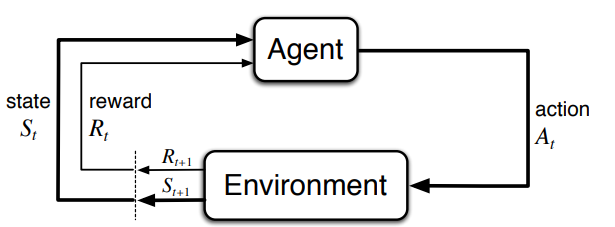
\includegraphics[width=0.75\linewidth]{Figures/Agent_Enviornment_Interaction.png}
         \caption{Agent Environment Interaction}
         \label{fig:enter-label}
     \end{figure}

    \begin{itemize}
        \item The Agent is the learner or decision maker.
        \item The agent Interacts with the environment selecting actions continually and the environment  responds back with different situations.
        \item The environment also  responds with  numerical  rewards in response to the action by the Agent .
    \end{itemize}
    
    The objective of the agent is to \textit{maximize} the \textit{total rewards} over time.
     
     \subsection{Markov Decision Process}
     Markov decision Process ( MDP) is a decision making mathematical model  that can address the Reinforcement learning Process.Markov decision Process ( MDP) follows the Markov property. The Markov property states that the future states of the system solely depends on the current state only and the History of the states is not required.
     
     As an example, lets consider a robot that is getting up from a chair and  making a step to move forward, The next state of the robot just depends on previous state (getting up to move) and not on the history ( sitting in chair). \cite{builtinUnderstandingMarkov}
     
     The MDP model comprises the following components.
     
     1.The set of Environment states $S$.
     
     2.The set of Actions $A$.
     
     3.The probability of state transitions represented as $P(s'|s,a)$ is the  probability of transitioning to state s' from state s given the likelihood action a.
     
     4.The reward signal at this time step $R(s,a)$ is reward collected at this time step as a result of taking a step a and this ending up in state s'.

     \noindent A Markov model is represented as a tuple of the above  $(S,A,P,R)$

     \noindent The transition probability P can be from state s to s' caused by action a  is 

     \begin{equation}
     P_{s,s'}^a = \mathbb{P}\{s_{t+1} = s' \mid s_t = s, a_t = a\}
    \end{equation}
     
     The reward signal for state s ,for an  action a at time step t is given by . 
     
     \begin{equation}
      R_{s,s'}^a = \mathbb{E}\{r_{t+1} \mid s_t = s, \\
     a_t = a, s_{t+1} = s'\}
     \end{equation}

     where E is the expected returns .

     \subsection{Policy and Value Functions:}
     
    "A \textit{policy} is a mapping from states to probabilities of selecting each possible
     action. If the agent is following policy $\pi$ at time t, then $p(a \mid s)$ is the probability that
     $A_t$ = a if $S_t$ = s." \cite{Sutton_Barto_2020}

    "The \textit{value function} of a state s under a policy $\pi$, denoted $v\pi(s)$, is the expected return
    when starting in s and following $\pi$ thereafter " \cite{Sutton_Barto_2020}

    \begin{equation}
    v_{\pi}(s) \doteq \mathbb{E}_{\pi} [G_t \mid S_t = s] = \mathbb{E}_{\pi} \left[\sum_{k=0}^{\infty} \gamma^k R_{t+k+1} \mid S_t = s \right], \quad \text{for all } s \in \mathcal{S},
    \end{equation}

    $E\pi$ denotes the expected value of a random variable given that the agent follows
    policy $\pi$, and t is any time step.

    "\textit{Action Value Function} $q_\pi$ defined as  the value of taking action a in state s under a policy $\pi$, denoted
    $q\pi(s, a)$, as the expected return starting from s, taking the action a, and thereafter
    following policy $\pi$:" \cite{Sutton_Barto_2020}
    
    \begin{equation}
     q_\pi(s, a) \doteq \mathbb{E}_\pi \left[ G_t \mid S_t = s, A_t = a \right] = \mathbb{E}_\pi \left[ \sum_{k=0}^{\infty} \gamma^k R_{t+k+1} \mid S_t = s, A_t = a \right]
    \end{equation}

    The largest expected return achievable by any policy for each state or state action pair is given by v* and q* respectively. This policy is called \textit{Optimal policy}.\cite{Sutton_Barto_2020}

    The Bellman optimality equation for $v^*$ can be given as :

   \begin{equation}
      v_*(s) = \max_a \sum_{s', r} p(s', r \mid s, a) \left[ r + \gamma v_*(s') \right]
   \end{equation}
  
    Similarly the Bellman optimality equation for $q^*$ can be given as : 
    
    \begin{equation}
    q_*(s, a) = \sum_{s', r} p(s', r \mid s, a) \left[ r + \gamma \max_{a'} q_*(s', a') \right]
   \end{equation}

     \subsection{Dynamic Programming}

     Dynamic programming is a technique in computer programming that involves breaking down an algorithmic problem into smaller sub-problems, saving their results, and then optimizing these sub-problems to determine the overall solution.\cite{bellman1966dynamic}

    Richard Bellman introduced dynamic programming in the 1950s. It is both a mathematical optimization method and a programming technique, particularly useful for problems that can be divided into overlapping sub problems or optimal substructures.

    In dynamic programming, overlapping sub problems occur when a larger set of equations is divided into smaller groups, and parts of these smaller equations are reused multiple times to arrive at the solution.
    
   In  Reinforcement Learning context, dynamic programming (DP) refers to a set of algorithms designed to compute optimal policies when provided with a perfect model of the environment, which is represented as a Markov decision process (MDP).\cite{Sutton_Barto_2020}

   Policy Iteration and Value iteration are the mostly used Dynamic programming Algorithms for obtaining optimal policies in Reinforcement Learning.

   \textit{Policy evaluation} is an iterative process used to calculate the value function for a given policy. \textit{Policy improvement} involves identifying a better policy based on the value function of the current policy. These two processes are integrated to form policy iteration and value iteration, which are the two most commonly used dynamic programming techniques.

   An important  characteristic of DP is \textit{bootstrapping} . This means, they update the state values based on the estimated values of the forthcoming states .

   \subsection{MonteCarlo Methods}
   Unlike dynamic programming, Monte Carlo methods do not require complete knowledge of the environment. Monte Carlo methods require only experience,they need a model .However the model doesn’t need to know the transition probabilities. It just needs to generate the sample sequences of states, actions, and rewards from actual or simulated interaction with an environment. It requires no prior knowledge of the environment’s dynamics.
    Montecarlo Methods solve the RL problem based on averaging the sample returns. The experiences from interaction is divided into episodes and these episodes has to eventually terminate irrespective of the actions selected. The Value estimates and subsequently the policy is updated only at the end of the episode \cite{Sutton_Barto_2020}

   \subsection{Temporal Difference Learning}
    Temporal Difference (TD) is a hybrid of both the Montecarlo and Dynamic programming.Like MonteCarlo, its Model free, meaning TD methods can learn directly from raw experience without a model of the environments dynamics.
    Like Dynamic Programming , TD algorithms bootstrap , meaning they update estimates based on other estimate and doesn’t wait for the episode to End.TD uses sample updates like Montecarlo.

     The simplest Temporal difference (TD) update can be shown as 

     \begin{equation}
    V(S_t) \leftarrow V(S_t) + \alpha \left[ R_{t+1} + \gamma V(S_{t+1}) - V(S_t) \right]
    \end{equation}

    At time \( t+1 \), make an update using the obtained reward ${R_{t+1}}$ and the value estimate ${V{s_{t+1}}}$

    \subsubsection{SARSA}
    SARSA is defined as on-policy TD Control to find optimal policy. SARSA stands for the transition given by State,Action,Reward,(next)State,(next)Action . This was proposed by Rummery and Nirajan  in article titled'"Modified Connectionist Q-Learning" (MCQ-L).'\cite{Rummery1994OnlineQU}

    The SARSA update equation is given below
    \begin{equation}
    Q(S_t, A_t) \leftarrow Q(S_t, A_t) + \alpha \left[ R_{t+1} + \gamma Q(S_{t+1}, A_{t+1}) - Q(S_t, A_t) \right]
    \end{equation}

     \noindent From the  state ${S_t}$,the agent chooses  ${A_t}$  , collects a reward ${R_{t+1}}$ , and goes to the next state ${S_{t+1}}$. The agent chooses the next action ${A_{t+1}}$ based on its policy ,collect the  action values at $Q({S_{t+1}}$,${A_{t+1}})$ and use it to estimate action values of the former state action $Q({S_t}$,${A_t})$.
     This update is done after every transition. 
     
     In SARSA the updates are made assuming we follow the actions defined by the policy. The policy used to make the Q value update and the one used to select next action is the same.Thus SARSA is online.The complete learning Algorithm is shown in the following table \cite{Sutton_Barto_2020}

    \begin{center}
    \begin{tabular}{|l|}
    \hline
    \textbf{Sarsa (on-policy TD control) for estimating $Q \approx q_*$} \\
    \hline
    Algorithm parameters: step size $\alpha \in (0, 1]$, small $\varepsilon > 0$ \\
    Initialize $Q(s, a)$, for all $s \in S^+$, $a \in \mathcal{A}(s)$, arbitrarily except that $Q(\text{terminal}, \cdot) = 0$ \\
    \textbf{Loop for each episode:} \\
    \hspace{1em} Initialize $S$ \\
    \hspace{1em} Choose $A$ from $S$ using policy derived from $Q$ (e.g., $\varepsilon$-greedy) \\
    \hspace{1em} \textbf{Loop for each step of episode:} \\
    \hspace{2em} Take action $A$, observe $R$, $S'$ \\
    \hspace{2em} Choose $A'$ from $S'$ using policy derived from $Q$ (e.g., $\varepsilon$-greedy) \\
    \hspace{2em} $Q(S, A) \leftarrow Q(S, A) + \alpha \left[ R + \gamma Q(S', A') - Q(S, A) \right]$ \\
    \hspace{2em} $S \leftarrow S'$; $A \leftarrow A'$; \\
    \hspace{1em} until $S$ is terminal \\
    \hline
    \end{tabular}
    \end{center}

    \subsubsection{Qlearning}
    Q-learning (Watkins, 1989) is a type of model-free reinforcement learning. It can also be considered a method of asynchronous dynamic programming (DP). This approach enables agents to learn how to act optimally in Markovian environments by experiencing the outcomes of their actions, without the need to construct explicit models or maps of the environment.Q learning is an offpolicy TD control.\cite{watkins1992q}
    
    The update equation for Q learning is 
     \begin{equation}
     Q(S_t, A_t) \leftarrow Q(S_t, A_t) + \alpha \left[ R_{t+1} + \gamma \max_{a} Q(S_{t+1}, a) - Q(S_t, A_t) \right]
     \end{equation}

     In Q learning ,the target policy is forced  to move towards the optimal policy $q^{*}$  by acting  greedily ($\underset{a}{max} Q({S_{t+1}},a)$) in that state .However the next Action by the Agent , is independent of the greedy action .Only the Q value update is made assuming we follow the greedy behaviour.Similar to asking the question. What is the estimate of $Q({S_t},{A_t})$ if we take a greedy action at this state ${S_{t+1}}$.The  rewards  $R_{t+1}$ are collected  for the initial action ${A_{t}}$ to compute the backed up action values for $Q({S_{t+1}},a)$, and used to estimate the values at $Q({S_t})$.

   Since both the behaviour and target policies are different , Q learning is  Off policy \cite{mnijuNotesQLearning}.The complete algorithm is shown below

   \begin{center}
   \begin{tabular}{|l|}
    \hline
    \textbf{Q-learning (off-policy TD control) for estimating $\pi \approx \pi_*$} \\
    \hline
    Algorithm parameters: step size $\alpha \in (0, 1]$, small $\varepsilon > 0$ \\
    Initialize $Q(s, a)$, for all $s \in S^+$, $a \in \mathcal{A}(s)$, arbitrarily except that $Q(\text{terminal}, \cdot) = 0$ \\
    \textbf{Loop for each episode:} \\
    \hspace{1em} Initialize $S$ \\
    \hspace{1em} \textbf{Loop for each step of episode:} \\
    \hspace{2em} Choose $A$ from $S$ using policy derived from $Q$ (e.g., $\varepsilon$-greedy) \\
    \hspace{2em} Take action $A$, observe $R$, $S'$ \\
    \hspace{2em} $Q(S, A) \leftarrow Q(S, A) + \alpha \left[ R + \gamma \max_{a} Q(S', a) - Q(S, A) \right]$ \\
    \hspace{2em} $S \leftarrow S'$ \\
    \hspace{1em} until $S$ is terminal \\
    \hline
    \end{tabular}
    \end{center}

    \subsection{Exploration and Exploitation dilemma}
    The trade off between exploration and exploitation is a challenging problem in reinforcement learning. To get maximum rewards, the agent must select the actions that it knows will produce high rewards. However in order to know which actions do drive high rewards, it has to  explore different actions and collect the rewards.The agent for some time must exploit the actions before starting to favour the actions that give high rewards. 

    One of the action selection rule used for exploration  is $\epsilon$ greedy method. In this method , the agent exploits taking  greedy action most of the time (1-$\epsilon$), except once a while with small probability $\epsilon$ the agent explores different actions.

    Contrast to this , the actions can also be selected  based on the probability of the available action values in a state also known as Softmax rule.

    \chapter{Related Work}
    \label{chap:rel_work}

    In cloud platforms, task consolidation is a effective means to manage resources.
    
    Lee et al \cite{lee2012energy} approaches this as a Task consolidation problem where the problem is the process of assigning n tasks to r cloud resources aiming to minimize the energy consumption by maximizing the resource utilization without violating the time constraints.
    They introduce two algorithms ECTC and MaxUtil . For any given tasks , the two heuristics check every resource and identify the energy efficient heuristic for that task .Its identified that the energy consumption difference between lower unutilized resource  and the higher utilized resource is not very significant and the difference is very high  between and idle resource and the underutilized resource. The cost function of ECTC algorithm tries to exploit this condition while the Maxutil cost function tries to improve the average utilization thus implicitly decreasing the number of active resources. The algorithm gives an impressive improvement of 18\% and 13\% respectively
    
    Srikkanth et al \cite{srikantaiah2008energy}argues that , the one of the major  causes of the energy in efficiency in data centre is the idle power wastage .They define two heuristics  for each server CPU usage and disk usage . At first from experiments, they identify the CPU usage and disk usage of the server that results the optimal disk utilization. In the next step, For each request received, an efficient bin packing is followed by using both the dimensions of the bin to the optimal point. A k dimensional Euclidean distance is calculated, to the optimal point along each dimension, which provides a scalar metric.  If this new request cannot be allocated in the server, then a new server is selected and the same heuristic is run there. This algorithm doesn't take into account of the multi tired applications or additional constraints like CPU and disk resources.
    
    Beloglazov et al \cite{beloglazov2012optimal} studies this more deeply. They split this is in three categories Host overload detection where the CPU utilization of the host is above the threshold, VM Selection the process of selecting the VM to migrate from the host once the Host becomes over loaded and VM placement. Three VM selection policies were proposed. Minimum migration policy (MMT) that migrates the VM that requires the minimum time for complete a migration. The random selection policy (RS)migrates a VM based on uniformly distributed random variable. In maximum correlation policy (MC) estimates the probability that a sever will overload assuming that there is higher correlation between the resource usage by applications.VM placement is the process of identifying a new host for the VM. This is treated similar to the bin packing problem. They propose a modified best fit decreasing (BFD) algorithm, and a modification of that is power aware BFD(PABFD) where the VM are sorted in the decreasing order of the current CPU utilizations, and then allocate the VM to the host that results in least increase in the power consumption. The authors conclude that the new policies outperform the existing policies.
    
    Ching et al \cite{hsu2011energy}introduces a new technique for task consolidation - ETC (Energy aware task consolidation) which aims to optimize energy consumption by defining ideal utilization thresholds of virtual machines. When the cpu utilization of the VM is lesser than the level, then the load is balanced within the cluster, else the tasks will be migrated to other resource with the minimal energy cost and execution cost. With simulation the authors were able to show that the ETC technique can reduce the energy consumption in task consolidation tasks by 17\%.
    
    Mogues \cite{moges2019energy} proposes a new bin packing algorithm Medium Fit (MF) that reduces the SLA violation and the number of VM migrations. The existing best fit (BF) and the first fit (FF) based algorithms results better efficiency but suffers from a limitation where there is a probability of higher overloading of the server. Medium Fit is introduced for this purpose. Two thresholds are defined one for over load and the other for underload. The average threshold is calculated from this and the MF algorithm favours the server whose desired utilization level has a minimum distance from the mean threshold. The MF rule with items sorted by decreasing size is called Medium Fit Decreasing (MFD)The experimental results from the authors show 67\% improvement in energy consumption and also reduction in SLA violation.
    
    Jinjiang \cite{wang2022research} proposes a VM consolidation method that is both energy efficient and have better Quality of service. They introduce a VM placement policy that searches the suitable host based on real time  cpu  utilization and power consumption. A VM selection Policy called AUMT is introduced, which selects the VMs with low average CPU utilization and migration time. Additional they propose different algorithms to detect Host over utilization and underutilization with Autoregressive Integrated moving model (ARIMA).By simulation with cloudsim, they were able to find that , the AUMT can reduce the energy usage by an average of 15.16 when compared to the MMT and MC
    
    Abdelkhalik et al \cite{mosa2019dynamic}proposes an energy aware virtual placement algorithm that is utility based and optimized for SLA. A model is developed for both the income and energy prediction.  The utility function runs a prediction of the income and energy cost of the virtual machines allocated to physical machines over time. A genetic algorithm based evolutionary approach is used for alternative search of VM to PM assignments. 
    The utility model tries to maximize the profit, that is derived from the income, energy cost and violation cost. The revenue that is made by the cloud provider by hosting the VMs is termed the income, the cost for the energy consumed by the VM placement termed as the energy cost and finally the violation cost is the penalty that gets paid from the host to the customer for the SLA violations. The utility model calculates and estimates the expected energy cost and the SLA violations that occurs due to the VM placement with the CPU utilization percentage. Next for VM placement, they propose genetic algorithm-based search and optimization technique as they have the ability to avoid the locally optimal solutions.
    The authors ran experiments in different scenarios to compare the performance of the proposed work and conclude that the Utility based solution saves more energy and reduces the SLA violations.

    \section{Machine Learning:}
    
    Fahimeh et al \cite{farahnakian2013lircup} tries to address the VM virtualization problem with Machine Learning. They propose a Linear Regression based algorithm to estimate the expected CPU usage of the host that predicts the overloading / underloading / status. The algorithm that forecasts the future CPU utilization is named Linear Regression based CPU Utilization Prediction (LiRCUP). When LirCUP predicts an overload, the VMS in the host will have to be migrated to a different host to avoid SLA violation, similarly, if LiRCUP forecasts underload in a host , some VMs migrate to other hosts so that the it can be switched to sleep mode to save energy. LirCUP algorithm approximates a prediction function using the relationship between the future and the current utilization of the host.
    
    Belgacem et al \cite{belgacem2023machine} introduces a VM migration-based learning model (VMLM) for the VM selection and VM migration. A classification model is built based on the data collected, with the required attributes (feature selection). The accuracy of the model is evaluated with cross validation before being implemented in the migration task. The model evaluates each migration to optimize for minimal energy consumption and migration time. This was able to achieve effective results compared to the classic algorithms like Minimum correlation (MC), Minimum migration Time (MMT) and Random Selection (RS)
    
    Portaluri et al \cite{portaluri2017power} introduces power efficient resource allocation algorithm for the cloud computing tasks. The algorithm Multi Objective Dynamic allocator (MODA) is based on Genetic Algorithm with multi objective optimization. The solution that that optimizes all the objectives at the same time is identified as the ideal vector. As part of the algorithm, non-dominated solutions are identified with number of power and energy related parameter are defined for the multi objective process. The solution with the least distance from the ideal vector is selected as the final optimized solution. 
    
    In 2015, Dashti et al \cite{dashti2016dynamic} proposed a modified version of the Particle Swarm Optimization (PSO) algorithm to dynamically optimize VM placement in data centers. Their goal was to increase the energy efficiency of data centers by optimizing VM placement. The main advantage of using PSO for VM placement is that it can dynamically optimize the placement of VMs in response to changes in the workload. This can help to improve the energy efficiency of the data center, while still meeting the performance requirements of the VMs.Dashti et al.'s approach used the Minimum Migration Time (MMT) metric to decide which VM to move from an over-utilized host. The host that the VM is to be placed on is then chosen using the PSO algorithm. The algorithm calculates a value for each potential placement based on the increase in power consumption from the new placement. The placement with the least increase in power consumption is chosen.
    
    Wei et al \cite{wei2010game}proposes Game theory to solve the resource allocation problem. They propose a twostep solution, where in first stage, the optimization problem is solved with Binary inter programming method independently and then in next stage based on the result in previous stage, an evolutionary optimization mechanism is proposed to obtain Quality of service and optimal energy usage.
    
    Deepika et al \cite{saxena2021proactive}proposes a framework for VM autoscaling approach where, the applicants resource requirement is predicted first and then this is matched with the resource capacity of the Virtual Machine, thus helping to keep the entire load requirement on the minimal number of the physical machines which is then followed by VM placement. An Evolutionary algorithm-based predictor model Online Multi Resource Feed Forward Neural Network (OM-FNN) is introduced to forecast the resource utilization. Additionally, another learning algorithm (TaDE) is developed that explores the population of solutions and selects the best solution. Auto scaling of the VMs is done by applying the K means clustering algorithm on the predicted resource utilization of tasks in different VMs. As for the VM placement, VMs are placed on energy efficient servers with maximum resource utilization and minimum power consumption using the multi objective VM placement approach.
    
    \section{Reinforcement Learning:}
    
    Das et al \cite{das2008autonomic}takes a muti agent approach for the power management of data centres. Their architecture has multiple separate agents and each agent interacts with other autonomous agents. In the end, a  multicriteria utility function estimates the joint utility function values of performance and power and based on that the physical severs are managed.
    
    Duggan et al \cite{duggan2016reinforcement}proposes Lr -RL a Reinforcement Learning   algorithm for VM selection problem. They propose a RL agent that is based on Q learning Algorithm. When a host is found to be over utilized, with the Lr algorithm, its placed in the list of Over utilised hosts. The host is selected one at a time from the list, the Lr -RL algorithm runs on it and then selects the VM to migrate from the current host to a suitable alternative host. Based on the Q learning algorithm the best optimal VM selection policy will be learnt. The RL algorithm reduces the energy consumption and number of migrations compared to the Lr-Mmt algorithm
    
    Shaw et al \cite{shaw2017advanced} proposes an RL based consolidation agent ( ARLCA) which learns the efficient policies for VM consolidation with no prior knowledge .ARCLA is a PBRS inspired RL technique , coupled with SARSA algorithm to  optimize the number of VMs in a host and ensures the host operates In an optimum resource usage.

    Quin et al \cite{qin2020virtual}proposes a multi objective reinforcement algorithm for the VM placement designed based on the Chebyshev scalarization function. They apply Pareto based RL algorithm successfully in the multi-objective setup which outperforms existing methods in most of the cases and has more scalability
    
    Farahnakian et al \cite{farahnakian2014energy} minimizes the number of active hosts in a cloud environment by using a Reinforcement Learning based dynamic consolidation method (RL-DC). The agent can use Q-learning algorithm to learn which power mode to set the host to in a given state, based on the current workload and other factors. To achieve this, the agent tries different actions (i.e., setting the host to different power modes) in different states and observes the results. It then adjusts its behaviour based on a penalty value that is calculated after all power mode changes. Over time, the agent learns to choose the best power mode for each state, which can help to minimize energy consumption and reduce SLA violations.
    
    Caviglione et al \cite{caviglione2021deep}formulate the VM placement problem as a multi-objective problem and propose an approximate approach based on DRL – Rainbow DQN to select suitable placement heuristics for each M.The results indicate that the proposed method outperforms bin packing heuristics commonly used in the literature for both synthetic and real workloads.
    
    Wei et al \cite{wei2023vmp}proposes another deep RL algorithm for the VM placement which is based on Asynchronous Advantage Actor critic algorithm VMP-A3C .Lr-Mmt is used for the   VM selection and Adaptive Three Threshold Energy Aware Algorithm to identify the workload status of Host Machines. A3C algorithm helps to map the VMs to the Host  Machines ( HM) .The convergence speed of VMP-A3C is better compared to other algorithms and it achieves better results.
	

	%There are two styles, depending on your sentence:
	%\begin{itemize}
	%\item Parenthetical \verb+\citep{NewmanGirvan2004}+: Community detection in graphs is an interesting problem \citep{NewmanGirvan2004}.
	%\item Textual \verb+\citet{NewmanGirvan2004}+: It was shown by \citet{NewmanGirvan2004} that community detection in graphs is an interesting problem.
	%\end{itemize}
	
		
	\chapter{Methodology}
	\label{chap:methodology}
 
        \section{Introduction:}
        To study and experiment with solutions to improve data center performance,a robust platform is required that enables the simulation of various conditions of datacentres in cloud computing  and testing of solutions within those scenarios. Also such a platform can help to benchmark and compare the algorithms against existing standard solutions.

        \section{The Simulation environment:Cloudsim}

        Cloudsim \cite{calheiros2011cloudsim} is a simulator that has been created by the CLOUDS laboratory in the university of Melbourne. Cloudsim toolkit is developed in Java that enables the modelling and simulation of the Cloud Computing environment. Cloudsim is used  to simulate the datacentre with different workloads and experiment with novel Algorithms .Cloudsim is a real bench marking toolkit in the field of Cloud simulation and many Algorithms are inbuilt into this including the LrMMT Algorithm which is the Gold standard benchmark  in this field.
        The tool is very modular in nature that provides the interfaces, to develop the required solutions. In this research solutions for VM selection algorithm is developed using cloudsim. Many researchers in this area cite Cloudsim in their benchmark study.

        \section{Cloudsim components}

        The CloudSim toolkit comprises a collection of Java classes and interfaces designed for defining and modeling various components within cloud environments, including data centers, virtual machines (VMs), applications, users, computing resources, and scheduling and provisioning algorithms. These elements can be customized, extended, or replaced to accommodate the simulation of specific cloud scenarios.\cite{calheiros2011cloudsim} Below is an overview of some essential classes and interfaces present in the CloudSim toolkit, which are consistent across all simulations:

        \textit{ICloudSim}: This is the main interface for initializing and managing the cloud environment within a simulation.

        \textit{DataCenter}:Represents a data center with its specific characteristics such as location, capacity, and power consumption.

        \textit{vm}:Represents a virtual machine with attributes like CPU, memory, and network bandwidth.

        \textit{Broker}:Acts as an intermediary between resource providers and users, managing the placement of applications on VMs and negotiating resource usage agreements.

        \textit{Application}:Represents the workload or application to be executed in the cloud environment, including its requirements for computational resources and deadline.

        \textit{Scheduler}: Manages the allocation of resources to applications based on specific scheduling policies.

        \textit{Resource}:Represents various computing resources such as CPU, memory, and network bandwidth available within a data center.
        
        \textit{Cloudlet}:Represents a single workload unit, with characteristics like processing requirements and deadline for completion.

        These fundamental components form the foundation of the CloudSim toolkit, enabling users to build sophisticated simulations of cloud environments while providing the flexibility to modify and extend individual elements as needed.

        \section{Cloudsim classes}

        The basic structure of the class hierarchy  is as shown in below class diagram  \cite{cloudsimtutorialsCloudSimSimulation}:

        \begin{figure}[H]
            \centering
            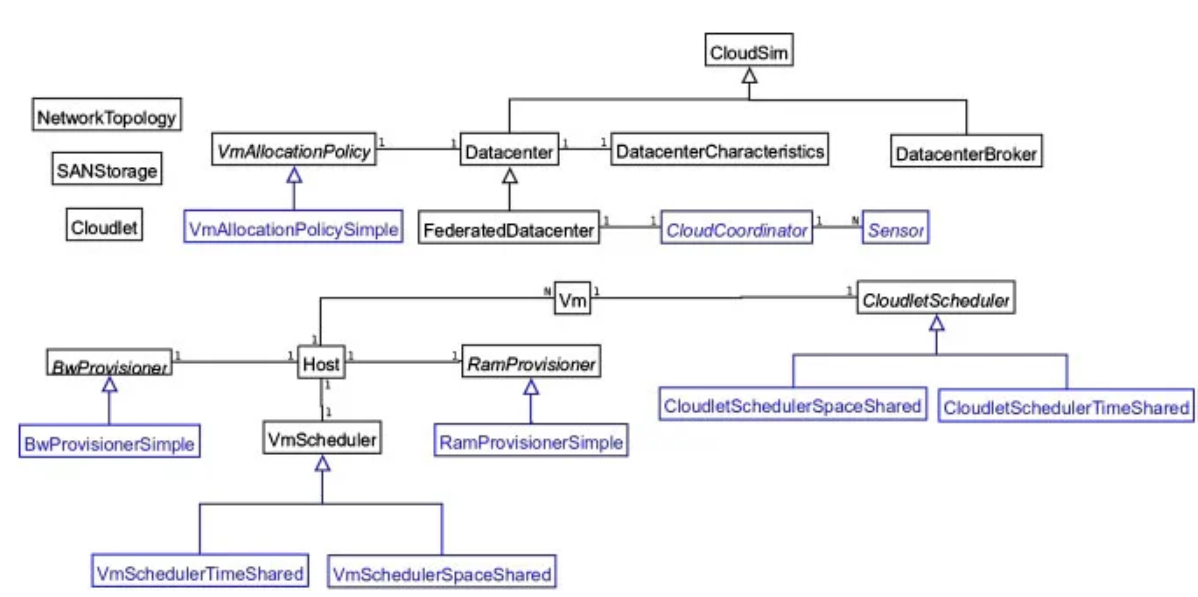
\includegraphics[width=1\linewidth]{Figures/Cloudsim_Class_Diagram.png}
            \caption{Cloudsim Class Diagram}
            \label{fig:Cloudsim class Diagram}
        \end{figure}
    
       Some of the important classes in the cloudsim Toolkit are briefed  below 

       \textit{\textbf{CloudSim}}This is the root class in the CloudSim toolkit. This class manages the simulation process and the event calls which are invoked during the simulation.

       \textit{\textbf{SimEntity}}: This is a very important class in the simulation process.All entities in CloudSim extends this class in order to be able to send events to other entities and also invoke event handlers to process incoming events during the simulation process. The three methods which are core to this class are \textit{startEntity()}, \textit{processEvent()} and \textit{shutdownEntity().}

       \textbf{\textit{SimEvent}}: This class models an event which is invoked by an entity and passed between two or more entities during the simulation process. This class encapsulates the details about an event such as the time the event should start and be delivered to the destination entity, data that must be passed with the event and also the event tag which is critical in order to identify the type of processing required by the event that has been sent and therefore it impacts directly on the resulting behaviour of an entity.

       \textbf{\textit{Datacenter}}: An instance of the datacenter class models the available hardware which is offered by the cloud provider. It encapsulates all of the hosts within the data center and is responsible for the implementation of a set of policies which governs the allocation of memory, bandwidth and storage devices to all hosts and their respective VMs.

       \textbf{\textit{Host}}: This class is used to model the server within the datacentre. The host stores information such as memory. The type of processing cores, allocation policies for sharing the VMs in the host and also the policies that govern the provisioning of memory and bandwidth of those VMs.

       \textbf{\textit{VM}}: This class represents the VMs in the host. The VMs are initialized with pre-defined memory , processing elements and size. The VMs are allocated the hosts based on the policies selected in the Host .

       \textit{\textbf{Cloudlet}}: This class is designed to represent the workload of application services in cloud computing environments. A cloudlet object essentially signifies the complexity level and computational demands of an application. To precisely simulate the stochastic nature of cloud environments, this class enables a cloudlet instance to acquire dynamic CPU utilization values instead of manually configuring cloudlet settings. In essence, it allows for more accurate modelling of real-world cloud conditions by incorporating variable CPU usage patterns.

       \textbf{\textit{DataCenterCharacteristics}}: This class embodies the properties and configuration of each data center such as OS , system architecture , list of hosts and type of VMM and the allocation policy being implemented.    

       \textit{\textbf{RamProvisioner:}}This abstract class can be used to define how the RAM (Random Access Memory) is allocated to the VM instances . RamProvisionerSimple policy is implemented by each host to allocate RAM to VMs from the host.

       \textit{\textbf{BwProvisioner:}}This  abstract class that can be used for provisioning bandwidth to the VMs. The default BwProvisioningSimple policy allows the host to allow maximum allocatable bandwidth for the host.

       \textbf{\textit{VmAllocationPolicy:}} This is the abstract class that can be used to define the policy for the allocation of the VMs to the Hosts . The main functionality of this class is to select a suitable host for the VM in the data centre from the list of over utilized hosts, based on the policy defined. 

       \section{Energy Aware Policy}
       Few of the standard energy aware policies like Lr-Mmt , Lr-Mc are readily available in the cloudsim toolkit \textit{org.cloudbus.cloudsim.examples.powerplanetlab } The VM Allocation policy and VM selection policies Abstract classes are defined in \textit{org.cloudbus.cloudsim.power}. The new VM selection or VM allocation policy defined must override these abstract classes to execute the respective algorithms.

       \section{Hardware setup }

       The CloudSim data center comprises 800 servers, each equipped with two cores, 4GB of RAM, and 1GB of storage and bandwidth per server. Additionally, CloudSim offers a variety of workloads that can be selected.The Host specification of datacenter  is specified  in file  \textit{org.cloudbus.cloudsim.examples.power/Constants.java}.Different Planetlab workloads are  also available that can be selected for running experiments .

       \chapter{Reinforcement Learning in Cloudsim}
       \label{chap:RL in Cloudsim}

       In this chapter we can see in detail the implementation of the RL Algorithm in clousdim. In particular we are interested in implementing the  VM selection policy using RL algorithm. This involves creating few classes that implements the interfaces to carry out VM selection.

       \section{RL VM Policy selection }
       In cloud sim , before we start the simulation, we define the  a new class which in turn will initiate the planetlab runner project .The required hyperparameters for the execution , the workload , the VM selection policy and , the VM Allocation policy are passed to planetlab runner project. The policies are passed as simple string value and based on this value , the respective policies are instantiated by the planetlabrunner().The planet lab runner object extends the RunnerAbstract() object .To select the reinforcement learning based VM selection policy in our experiments, the string \textit{'RL’} is passed in the planet lab runner as VM selection policy . The runner abstract has a method getVmSelectionPolicy() .If the vmSelectionPolicyName is “RL” then the method getVmSelectionPolicy() from RunnerAbstract class instantiates  PowerVmSelectionPolicyReinforcementLearning() policy.

       \section{PowerVMSelectionPolicy} 
       This is the policy that will be utilized to select the VMs to move  from a host when the host is overutilized. Essentially, we have objects of type \textit{Environment, Agent} and \textit{Algorithm} as part of the new RL algorithm implementation. The method getVmToMigrate() will be called from the getVmsToMigrateFromHosts() in the PowerVmAllocationPolicyMigrationAbstract class .The getVmToMigrate()  method will be over-ridden by the PowerVMSelectionPolicy Reinforcement Learning class. This method gets the  Vms to be selected from the current host by calling the getAction() method in the Agent class.

       \section{Agent}
       The agent here refers to the RL Agent that interacts with other components  in cloudsim. The Agent class includes two key methods getAction() and updateQValues() , with getAction() being the primary one. getAction() calls the Migrate() method from the Algorithm class.\cite{Lukethesis} It is crucial to note that migration must take place before updating the Q values. A DataCenter event, is triggered by the run() method in simEntity class .A process event is generated every 300ms from updateCloudletProcessingReinforcementLearning() method in PowerDataCenter class , which initiates the whole  process.The event starts with the check for over-utilized hosts using Local Regression algorithm(a VM Allocation Policy) in the optimizeAllocationRL() method in PowerVmAllocationPolicyMigrationAbstract class.The Lr in Lr-RL stands for Local Regression. For each over utilized host, the getVmToMigrate() method in  PowerVmSelectionPolicyRL class calls the agent class, which in turn calls the migrate method in the algorithm class. Once migration is completed, an event is triggered to call updateQValues() in PowerVmSelectionPolicyRL class and subsequently in the Agent class. Depending on the employed algorithm, the algorithm then updates the Q-Value. A check is conducted to determine if the host still remains over-utilized; if it does, the VM migration process resumes. This process  continues  for each over-utilized host.

       \begin{figure}[H]
           \centering
           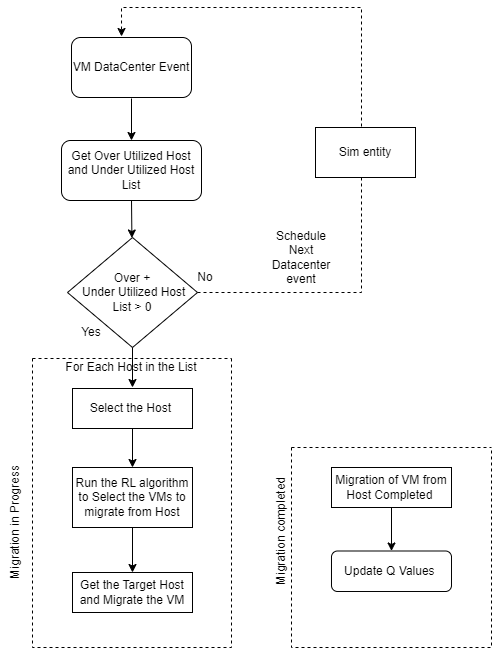
\includegraphics[width=1.0\linewidth]{Figures/VM_Migration.png}
           \caption{ Reinforcement Learning Algorithm in Cloudsim}
           \label{fig:enter-label}
       \end{figure}

       \section{Algorithm}
       As the name mentions, the algorithm class has the algorithm to choose the VMs to migrate from the over utilized host. We use Q learning or SARSA  algorithm to Update the Q values of the Vms based on the initial section.The algorithm has the methods SARSAUpdateQValues() and QLearningUpdateQValues() to update the Q values .The Algorithm class has the attributes like Q values, reward, current state and next state.The agent gets these information from the environment class.

       \section{Environment class}
       The environment stores the methods and attributes to be shared with the agent and the algorithm. This class has the methods to discretize the states, calculate the rewards and also stores the Q values for the state action pair. The agent interacts with the cloudsim toolkit, gets the reward , calculates the Q value for the state action pair and its updated to the Environment.

       \section{LrRL}
       The LrRL class is placed in the folder \textit{org.cloudbus.cloudsim.examples.power.planetlab}  along with all of the other Energy Aware Policies. The class has a main method, that initiates the Algorithm class, Agent class, sets the policy hyperparameters ,VMAllocationPolicy, VM selectionPolicy , simulation workload and then instantiates a PlanetLabRunner object. The runner abstract has a method getVmSelectionPolicy() .If the vmSelectionPolicyName is “RL” then the policy PowerVmSelectionPolicyReinforcementLearning is selected. In this research we also have VM Allocation set to Lr, which means Local Regression . Executing  this will run the simulation with VM Allocation policy set to the inbuilt Local Regression Algorithm and the Vm selection as the Reinforcement Learning policy cobinely called Lr-RL.\cite{Lukethesis}

       \section{VM Selection Process:}
       The simulator has the VM DataCenter event triggered once every 300 seconds. This in turn calls a series of methods as shown in the flowchart (figure 6.2t) hat will first check the overutilized hosts and then for each over utilized host, the RL algorithm selects the VMs that can be migrated to another host. After migration, again a check is done if the host is overutilized or underutilised. This process of selecting a VM from a host and migrating the VM to a target host continues for all the over utilized hosts. Once this cycle is completed and VM datacenter event is again triggered in 300 seconds.

       \begin{figure}[H]
           \centering
           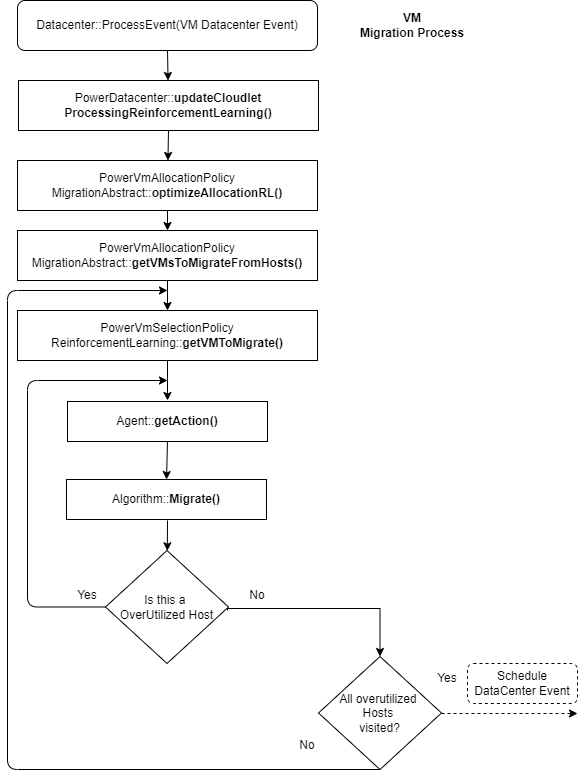
\includegraphics[width=1.0\linewidth]{Figures/VM selection Process.png}
           \caption{VM Selection Lr-RL}
           \label{fig:enter-label}
       \end{figure}

       
       \section{Q Value Update Process:}
       This method is part of the Agent Class. This method is called  as part of the VM migration process after the VM migration process  is completed .
       Its invoked by calling, agent.Updateqvalues() method. Based on the algorithm selected in algorithm class , either Q learning or SARSA be executed . Both Q learning and SARSA are  implemented in the algorithm class. The Q values are updated for each state action pair.

       \begin{figure}[H]
           \centering
           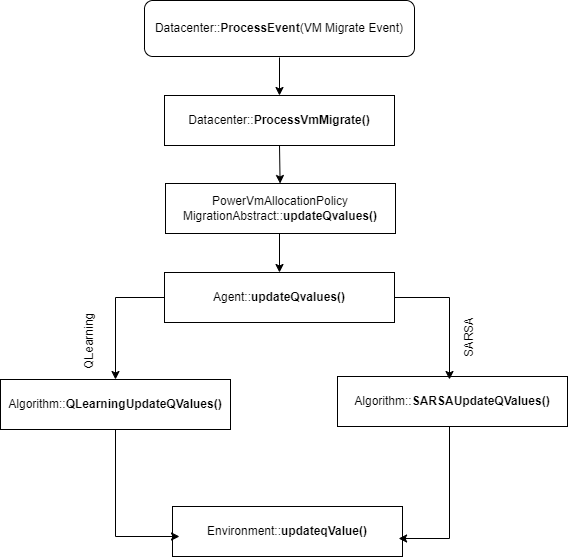
\includegraphics[width=0.75\linewidth]{Figures/UpdateProcess.png}
           \caption{Lr-RL update Q values}
           \label{fig:enter-label}
       \end{figure}

       \section{State-Action Space}
       Defining the state action space in a complex domain like cloud computing is daunting. The RL setup needs proper definition of state action space for its execution. The Q learning algorithm that we use is a discrete algorithm and we need to discretize the continuous variables so as to avoid any curse of dimensionality. The state space is defined to have states and actions for every 1 \% for the range of 0 to 100\%. The state space is defined with the Host Utilization. The sum of CPU usage of all the VMs divided by the total Host Mips. Sometimes the host is given a state value above 100 to accommodate a state value above 100\%, The state values are rounded integers. Based on the experimental logs of the state its decided to have 301 states .\cite{Lukethesis}

      \begin{equation}
       s = \frac{\sum_{k=1}^{k} VMcpu(k)}{Hcpu} \cdot 100
      \end{equation}

      VMcpu here represents the total utilization of the VMs in the Host and Hcpu is the total Host utilization.
      
    The action space is defined just with the VM utilization. Here the ratio of the utilization of a VM in relative to the combined utilization of all the VMs is calculated and the integer value is rounded to an integer between 1-100 .Totally there are 101 actions.
    
    \begin{equation}
    a = \frac{VMa}{\sum_{k=1}^{k} VMcpu(k)} \cdot 100
    \end{equation}

   VMa represents the utilization of the VM and k represents all the VMs in the host . VMcpu represents the VM utilization in the host.

   \section{Reward}
   The reward is designed so at to facilitate few migrations. This would greatly reduce the energy consumption. To encourage fewer migrations, instead of migrating many smaller VMs , few larger VMs should be migrated, The reward encourages the actions with large action value ( bigger VMs are prioritized over smaller VMs). Moving large VMs is expected to result with  the host spending less time overutilized and therefore the SLAVs is also expected to improve.

    \section{Q Learning}
    Q learning is a Tabular model free algorithm.Its an off policy TD ( Temporal Difference) control. The Q learning algorithm is run over each over utilized hosts to select the VMs for migrate. Initially , the current state of the over utilized host is observed. All the VMs of the host are iterated over and their action values are calculated and this is updated to form the state action list.  The action with the largest Q values is selected. If there are multiple VMs with same Q values, one is selected randomly. The chosen action is the VM selected to be migrated . Once the migration is completed, the next state and the reward for the action are observed and the Q values are update for that state.The algorithm for Q-Learning update is shown below\cite{Lukethesis}

    \begin{center}
    \begin{tabular}{|l|}
    \hline
    \textbf{Algorithm: Q-Learning Algorithm for VM Selection} \\
    \hline
    \textbf{for all} Hosts in Over-Utilized Host List \textbf{do} \\
    \hspace{1em} \textbf{while} Host is Over-Utilized \textbf{do} \\
    \hspace{2em} \textbf{Observe} Current State (Host Utilization \%)\\
    \hspace{2em} \textbf{for all} VMs on the Over-Utilized Host \textbf{do} \\
    \hspace{3em} \textbf{Get} Action Value for VM \\
    \hspace{2em} \textbf{end for} \\
    \hspace{2em} \textbf{for all} VM Action Values \textbf{do} \\
    \hspace{3em} \textbf{Lookup} Q-Value for (Current State, Action) Pair \\
    \hspace{2em} \textbf{end for} \\
    \hspace{2em} \textbf{Choose} VM with highest Q-Value \\
    \hspace{2em} \textbf{Migrate} VM \\
    \hspace{2em} \textbf{Observe} Next State, Reward \\
    \hspace{2em} \textbf{Get} maxQ - The maximum Q-Value in the Next State \\
    \hspace{2em} \textbf{Calculate} $newQ = previousQ + \alpha * [reward + \gamma * maxQ - previousQ]$ \\
    \hspace{2em} \textbf{Update} Q(s,a) with new value \\
    \hspace{1em} \textbf{end while} \\
    \textbf{end for} \\
    \hline
    \end{tabular}
    \end{center}

    \section{SARSA}

    SARSA algorithm unlike Q learning is an online algorithm .This means both the target policy and the behavioural policy are the same.The Q value is calculated in this algorithm following the same steps in Q Learning . However, in the Q value update  step instead of taking the max action value,of the next state in Q learning, SARSA  uses  the next action value of the next state it follows to calculate the next state Q value.This is the key difference between the two algorithms.The algorithm for SARSA update is shown below\cite{Lukethesis}

     \begin{center}
    \begin{tabular}{|l|}
    \hline
    \textbf{Algorithm: SARSA Algorithm for VM selection} \\
    \hline
    \textbf{for all} Hosts in Over-Utilized Host List \textbf{do} \\
    \hspace{1em} \textbf{while} Host is Over-Utilized \textbf{do} \\
    \hspace{2em} \textbf{Observe} Current State (Host Utilization \%) \\
    \hspace{2em} \textbf{for all} VMs on the Over-Utilized Host \textbf{do} \\
    \hspace{3em} \textbf{Get} Action Value for VM \\
    \hspace{2em} \textbf{end for} \\
    \hspace{2em} \textbf{for all} VM Action Values \textbf{do} \\
    \hspace{3em} \textbf{Lookup} Q-Value for (Current State, Action) Pair \\
    \hspace{2em} \textbf{end for} \\
    \hspace{2em} \textbf{Choose} VM with highest Q-Value \\
    \hspace{2em} \textbf{Migrate} VM \\
    \hspace{2em} \textbf{Observe} Next State, Reward \\
    \hspace{2em} \textbf{for all} VMs on the Host \textbf{do} \\
    \hspace{3em} \textbf{Get} Action Value for VM \\
    \hspace{2em} \textbf{end for} \\
    \hspace{2em} \textbf{Choose} VM with highest Q-Value \\
    \hspace{2em} \textbf{Get} QVal - The Q-Value of the (Next State, Next Action) Pair \\
    \hspace{2em} \textbf{Calculate} $newQ = previousQ + \alpha * [reward + \gamma * QVal - previousQ]$ \\
    \hspace{2em} \textbf{Update} Q(s,a) with new value \\
    \hspace{1em} \textbf{end while} \\
    \textbf{end for} \\
    \hline
    \end{tabular}
    \end{center}


   \chapter{Evaluation Benchmarks }
   \label{chap:Evaluation Benchmarks}

    \section{Introduction:}
    This chapter gives an overview of the performance metrics used in this study.Metrics commonly employed for benchmarking in relevant journals are examined and applied to evaluate the algorithms in this thesis.

    
   \section{Metrics}
   \subsection{DataCenter energy consumption}
    This is a key performance metric as the key research criteria is to reduce the energy consumption of data centers,The metric is Kilowatthours(kWh). 

    \subsection{VM Migrations:}
    Another key research criteria in this topic is aimed to reduce the number of VM migrations by using reinforcement learning algorithms for VM selection policy. A reduction in the number of VM migrations is good sign the RL based Vm selection policy is working as intended. Reduced migrations is expected to improve Energy efficiency .

    \subsection{Service level Agreement Violations (SLAVs):}
    A robust SLA is the foundation to establish a better operative sevice on the cloud. A reduction in the energy may reduce the Quality of Service (QOS) provided and this is not desired.Therefore a balance must be maintained between the Energy reduction and the SLAs to maintain better quality service . This metric is derived from two parameters , Performance Degradation Due to Migrations (PDM) and Service Level Agreement Violation Time Per Active Host (SLATAH).  the SLAV is calculated by multiplying the SLATAH with the PDM.
        \begin{equation}
        SLAV = SLATAH. PDM
        \end{equation}
        
    \subsection{Performance Degradation Due to Migrations  (PDM)}
     This metric gives the  drop in performance when moving the VM from one host to another host (Vm migrations) 
     \begin{equation}
    PDM = \frac{1}{M} \sum_{k=1}^{M} \frac{C_{dj}}{C_{rj}}
    \end{equation}

    M represents the number of VMs, $C_{di}$ represents an estimate of how much the performance of VM \textit{j} is reduced due to migrations, and $C_{rj}$ represents the lifetime requested CPU capacity by VM \textit{j}.

    \subsection{Service Level Agreement Violation Time Per Active Host (SLATAH)}
     The VMs are unlikely to run with optimal performance in a over utilized host. This parameter just captures the actual time the host run at full capacity in its total runtime .
    H represents the number of hosts, $T_{sk}$ is equal to the total time host k spends at maximum utilization and $T_{ak}$ is the total time that host is active.

    \begin{equation}
    SLATAH = \frac{1}{H} \sum_{k=1}^{H} \frac{T_{sk}}{T_{ak}}
    \end{equation}

    \subsection{Energy and SLAV - combined Metric:}
    As discussed in previous sections, the energy and the SLAV have inverse relationship, however they both are essential for evaluating the datacenter performance. A metric that combines both these metrics that can help to evaluate the algorithm performance. ESV is defined as the product of the two parameters EC and SLAV as shown below

    \begin{equation}
     ESV = EC. SLAV 
     \end{equation}

    
    \chapter{Discount Factor Vs Learning Rate}
    \label{chap:hyperparams}
 
      \section{Introduction:}
      In this section the comparison between the two hyperparameters alpha and gamma used in Q learning and sarsa is evaluated. Learning rate is noted as $\alpha$ and the discount factor as $\gamma$ in the equation used for Q value update.
      The parameters that yield the minimal energy consumption, migrations and ESV are analysed over 30 day average and finally the best values for these two hyper parameters are discussed for these two algorithms . 

      \section{Experimental Setup:}
      
      Cloudsim simulator will be used to simulate the data center and planetlab workload data set will be used to run the experiments.Each planetlab workload comprises of a file with CPU usage .It consists of 288 values , the CPU Usage percentage values for every 5 minutes . Executing the cloudsim with one work load file accounts for running the simulation for 24 hours  . In order to come to any formal conclusion the experiments  need to be run for 30 days . A 30 day workload is created randomly selecting from the existing planet lab workload.The Number of hosts is fixed to be at 800. The no of VMs for the day is defined by the number of workload files for the day available in the planet lab dataset.

      The experiment is conducted using two algorithms, Q-learning and SARSA, with each algorithm tested under two action selection policies: epsilon-greedy and Softmax. In total, the following combinations are explored.
      
      \begin{enumerate}
      \item Q-learning with $\epsilon$-greedy action
      \item Q-learning with softmax action
      \item SARSA with $\epsilon$-greedy action
      \item SARSA with softmax action
      \end{enumerate}
      
      For each algorithm listed above hyperparameter sweep will be done for both the learning rate alpha and the discount factor gamma.

      The Alpha an Gamma  values chosen for the parameter experiment are shown below :

      \begin{table}[h!]
        \centering
        \begin{tabular}{|c|c|c|c|c|c|c|}
        \hline
        \textbf{Learning rate $\alpha$ } & 0.2 & 0.4 & 0.6 & 0.8 & 0.9 & 1.0 \\
        \hline
        \textbf{Discount Factor $\gamma$} & 0.2 & 0.4 & 0.6 & 0.8 & 0.9 & 1.0 \\
        \hline
        \end{tabular}
        \caption{$\alpha$ and $\gamma$ values}
        \end{table}

       For each experiment listed above, with the hyper parameter combination of alpha and gamma sweeps, there will be total 36 experiment results  for the 30 day period.To allow the agent to learn from the previous experience , the q values learnt in day one is passed to the next day .However its reset at the end of each parameter sweep. The 30 day data collected is then averaged for each hyperparameter combination for the analysis.

       \section{Q-learning - $\epsilon$ greedy:}
        The details collected from the parameter sweep of learning rate and discount factor is shown in table 8.2 below. The Energy consumption is mostly proportional to the  VM migrations. The minimal Energy consumption of 141.63 kWh occurred at the alpha value of 1.0 and gamma value of 0.2.
        
        Its observed the higher values of learning rate improves the energy efficiency . However the gamma values didn't have much of any influence on the results. The ESV and no of VM  migrations are low at alpha 0.8 and gamma 0.2 .The energy consumption at this combination is 141.65 kWh, slightly hgher than the combination with alpha 1.0 and gamma 0.2. The ESV is the minimal at 0.00989.

        From the table below, it can be  observed that its desirable to have higher learning rate and a lower discount rate. This explains  the agent would like to learn faster , at the same time,the lower gamma values indicates that the agent prioritizes immediate rewards over future rewards.

       \begin{table}[H]
        \centering
        \small
        \begin{tabular}{|c|c|c|c|c|c|}
        \hline
        \textbf{Alpha} & \textbf{Gamma} & \textbf{Energy (kWh)} & \textbf{Total Migrations} & \textbf{SLAV(\%)} & \textbf{ESV} \\ 
        \hline
        0.2 & 0.2 & 142.91258 & 17844 & 0.00728 & 0.010404 \\ 
        0.2 & 0.4 & 142.81709 & 18012 & 0.007281 & 0.01039 \\ 
        0.2 & 0.6 & 143.80451 & 19324 & 0.007452 & 0.01071 \\ 
        0.2 & 0.8 & 146.58258 & 21390 & 0.007802 & 0.01143 \\ 
        0.2 & 0.9 & 150.14322 & 23216 & 0.008073 & 0.01212 \\ 
        0.2 & 1.0 & 169.45354 & 27734 & 0.007083 & 0.01200 \\ 
        0.4 & 0.2 & 142.21677 & 17281 & 0.007160 & 0.01018 \\ 
        0.4 & 0.4 & 142.31935 & 17672 & 0.007149 & 0.01017 \\ 
        0.4 & 0.6 & 143.07516 & 18555 & 0.007255 & 0.01038 \\ 
        0.4 & 0.8 & 145.93064 & 20984 & 0.007812 & 0.01140 \\ 
        0.4 & 0.9 & 148.14483 & 22340 & 0.008121 & 0.01203 \\ 
        0.4 & 1.0 & 162.35419 & 26556 & 0.007738 & 0.01256 \\ 
        0.6 & 0.2 & 141.84032 & 16781 & 0.00703 & 0.009971 \\ 
        0.6 & 0.4 & 142.04064 & 17326 & 0.00710 & 0.010089 \\ 
        0.6 & 0.6 & 142.79387& 18178 & 0.007261 & 0.01036 \\ 
        0.6 & 0.8 & 144.43806 & 19714 & 0.00755 & 0.01091 \\ 
        0.6 & 0.9 & 146.91064 & 21400 & 0.00790 & 0.01162 \\ 
        0.6 & 1.0 & 163.34354 & 26630 & 0.00784 & 0.01280 \\ 
        \textbf{0.8} & \textbf{0.2} & \textbf{141.6558} & \textbf{\textcolor{red}{16590}} & \textbf{0.00698} & \textbf{\textcolor{red}{0.00988}} \\ 
        0.8 & 0.4 & 141.89354 & 17155 & 0.007036452 & 0.00998 \\ 
        0.8 & 0.6 & 142.54193 & 17853 & 0.007190645 & 0.01024 \\ 
        0.8 & 0.8 & 144.08870 & 19201 & 0.007504516 & 0.01081 \\ 
        0.8 & 0.9 & 145.50193 & 20342 & 0.007822903 & 0.01138 \\ 
        0.8 & 1.0 & 161.25451 & 26212 & 0.008332258 & 0.01343 \\ 
        0.9 & 0.2 & 141.63935 & 16694 & 0.007046774 & 0.00998\\ 
        0.9 & 0.4 & 141.84677 & 17025 & 0.007054194 & 0.01000\\ 
        0.9 & 0.6 & 142.49387 & 17810 & 0.007190645 & 0.01024\\ 
        0.9 & 0.8 & 143.71806 & 18832 & 0.007435161 & 0.01068\\ 
        0.9 & 0.9 & 144.63032 & 19655 & 0.007618065 & 0.01101\\ 
        0.9 & 1.0 & 161.02096 & 25987 & 0.008249355 & 0.01328\\ 
        \textbf{1.0} & \textbf{0.2} & \textbf{\textcolor{red}{141.6338}} & \textbf{16631} & \textbf{0.00700} & \textbf{0.00992} \\ 
        1.0 & 0.4 & 141.79322 & 16932 & 0.00700871 & 0.009937 \\ 
        1.0 & 0.6 & 142.50451 & 17689 & 0.007152258 & 0.01019 \\ 
        1.0 & 0.8 & 143.78193 & 19002 & 0.007414839 & 0.01066\\ 
        1.0 & 0.9 & 144.59806 & 19677 & 0.007543548 & 0.01090 \\ 
        1.0 & 1.0 & 163.17548 & 26635 & 0.007419677 & 0.01210 \\ 
        \hline
        \end{tabular}
        \caption{Qlearning $\epsilon$ greedy: 30 day average of Energy Consumption, Total Migrations, SLAV\%, and ESV values  }
        \end{table}

     
        \section{Q-learning - softmax:}

        The results of this experiment is shown in the following table 8.3. As in the previous experiment , the lower energy Consumption occurs for the parameter alpha 1.0 and gamma 0.2. Unlike in the qlearning with $\epsilon$ greedy,in this experiment the lowest migrations and ESV all happen in this specific combination. The lowest energy consumption is 141.97 kwh which is slightly more than the previous experiment qlearning with $\epsilon$ greedy. The total migration count is also 17065 which is higher than the  $\epsilon$ greedy variant . Consequently the ESV is also higher than the previous experiment.

        With the hyperparmeter values learning rate 1.0 and discount factor 0.2 ,the best agent likes to  learn aggressively with lesser significance to previous learnt values.

        \begin{table}[H]
        \centering
        \small
        \begin{tabular}{|c|c|c|c|c|c|}
        \hline
        \textbf{Alpha} & \textbf{Gamma} & \textbf{Energy (kWh)} & \textbf{Total Migrations} & \textbf{SLAV(\%)} & \textbf{ESV} \\ 
        \hline
        0.2 & 0.2 & 143.01000 & 17993 & 0.00729 & 0.01043 \\ 
        0.2 & 0.4 & 142.82742 & 18101 & 0.00728 & 0.01040 \\ 
        0.2 & 0.6 & 143.97935 & 19448 & 0.00751 & 0.01082 \\ 
        0.2 & 0.8 & 146.72613 & 21656 & 0.00783 & 0.01149 \\ 
        0.2 & 0.9 & 151.55581 & 23945 & 0.00796 & 0.01206 \\ 
        0.2 & 1.0 & 166.72000 & 27289 & 0.00722 & 0.01204 \\ 
        0.4 & 0.2 & 142.46548 & 17472 & 0.00719 & 0.01024 \\ 
        0.4 & 0.4 & 142.75935 & 18079 & 0.00724 & 0.01033 \\ 
        0.4 & 0.6 & 143.75613 & 19277 & 0.00746 & 0.01072 \\ 
        0.4 & 0.8 & 145.88742 & 20970 & 0.00780 & 0.01138 \\ 
        0.4 & 0.9 & 148.46419 & 22558 & 0.00808 & 0.01200 \\ 
        0.4 & 1.0 & 162.55161 & 26551 & 0.00760 & 0.01236 \\ 
        0.6 & 0.2 & 142.19613 & 17261 & 0.00708 & 0.01007 \\ 
        0.6 & 0.4 & 142.66355 & 18046 & 0.00722 & 0.01030 \\ 
        0.6 & 0.6 & 143.36516 & 18833 & 0.00734 & 0.01052 \\ 
        0.6 & 0.8 & 145.32935 & 20566 & 0.00775 & 0.01126 \\ 
        0.6 & 0.9 & 147.12226 & 21666 & 0.00797 & 0.01173 \\ 
        0.6 & 1.0 & 160.45774 & 26136 & 0.00779 & 0.01251 \\ 
        0.8 & 0.2 & 142.05935 & 17145 & 0.00707 & 0.01005 \\ 
        0.8 & 0.4 & 142.42129 & 17675 & 0.00715 & 0.01018 \\ 
        0.8 & 0.6 & 143.03806 & 18496 & 0.00731 & 0.01046 \\ 
        0.8 & 0.8 & 144.49097 & 19733 & 0.00759 & 0.01097 \\ 
        0.8 & 0.9 & 145.57323 & 20508 & 0.00781 & 0.01136 \\ 
        0.8 & 1.0 & 158.33129 & 25573 & 0.00812 & 0.01286 \\ 
        0.9 & 0.2 & 142.17774 & 17216 & 0.00717 & 0.01019 \\ 
        0.9 & 0.4 & 142.39677 & 17656 & 0.00721 & 0.01026 \\ 
        0.9 & 0.6 & 142.90645 & 18179 & 0.00726 & 0.01038 \\ 
        0.9 & 0.8 & 144.28065 & 19421 & 0.00756 & 0.01090 \\ 
        0.9 & 0.9 & 145.20000 & 20021 & 0.00773 & 0.01122 \\ 
        0.9 & 1.0 & 153.78742 & 24282 & 0.00817 & 0.01256 \\ 
        \textbf{1.0} & \textbf{0.2} & \textbf{\textcolor{red}{141.97839}} & \textbf{\textcolor{red}{17065}} & \textbf{\textcolor{red}{0.00707}} & \textbf{\textcolor{red}{0.01004}} \\ 
        1.0 & 0.4 & 142.21613 & 17377 & 0.00709 & 0.01008 \\ 
        1.0 & 0.6 & 142.70968 & 17932 & 0.00720 & 0.01028 \\ 
        1.0 & 0.8 & 143.72677 & 18845 & 0.00738 & 0.01061 \\ 
        1.0 & 0.9 & 144.29290 & 19464 & 0.00760 & 0.01096 \\ 
        1.0 & 1.0 & 153.37735 & 24101 & 0.00817 & 0.01253 \\ 
        \hline
        \end{tabular}
        \caption{Qlearning softmax: 30 day average of Energy Consumption, Total Migrations, SLAV\%, and ESV values}
        \end{table}

        \section{SARSA - $\epsilon$ greedy:}

        The table 8.4 from the parameter sweep of learning rate and discount factor is shown below .  The minimal Energy consumption of 141.30 kWh occurred at the alpha value of 0.6 and gamma value of 0.4.
        
        Similar to earlier experiments , Its observed the higher values of learning rate improves the energy consumption . However the gamma values didn't have much of any influence on the results. The ESV and no of migrations are low at alpha 0.8 and gamma 0.2 as highlighted in table.The energy consumption at this combination is 141.34 kWh. The difference in energy consumption between this   and the one mentioned above is just 0.04 kWh. The ESV is the minimal at 0.00973

        The energy consumption,migration count and  ESV in SARSA epsilon is slightly less than the experiment with Q learning epsilon .

        \begin{table}[H]
        \centering
        \small
        \begin{tabular}{|c|c|c|c|c|c|}
        \hline
        \textbf{Alpha} & \textbf{Gamma} & \textbf{Energy (kWh)} & \textbf{Total Migrations} & \textbf{SLAV (\%)} & \textbf{ESV} \\ 
        \hline
        0.2 & 0.2 & 142.076129 & 17123 & 0.00715 & 0.01016 \\ 
        0.2 & 0.4 & 141.3880645 & 16429 & 0.00691 & 0.00977 \\ 
        0.2 & 0.6 & 141.3845161 & 16437 & 0.00693 & 0.00980 \\ 
        0.2 & 0.8 & 141.4677419 & 16491 & 0.00695 & 0.00983 \\ 
        0.2 & 0.9 & 141.4754839 & 16505 & 0.00697 & 0.00986 \\ 
        0.2 & 1.0 & 141.4993548 & 16574 & 0.00695 & 0.00984 \\ 
        0.4 & 0.2 & 141.3254839 & 16401 & 0.00694 & 0.00980 \\ 
        0.4 & 0.4 & 141.3464516 & 16420 & 0.00692 & 0.00979 \\ 
        0.4 & 0.6 & 141.4232258 & 16467 & 0.00694 & 0.00982 \\ 
        0.4 & 0.8 & 141.4441935 & 16470 & 0.00692 & 0.00979 \\ 
        0.4 & 0.9 & 141.4964516 & 16605 & 0.00694 & 0.00982 \\ 
        0.4 & 1.0 & 141.6180645 & 16658 & 0.00699 & 0.00990 \\ 
        0.6 & 0.2 & 141.3619355 & 16409 & 0.00692 & 0.00978 \\ 
        \textbf{0.6} & \textbf{0.4} & \textbf{\textcolor{red}{141.30483}} & \textbf{16400} & \textbf{0.00691} & \textbf{0.00977} \\ 
        0.6 & 0.6 & 141.4890323 & 16575 & 0.00697 & 0.00986 \\ 
        0.6 & 0.8 & 141.5496774 & 16577 & 0.00695 & 0.00983 \\ 
        0.6 & 0.9 & 141.6864516 & 16719 & 0.00701 & 0.00993 \\ 
        0.6 & 1.0 & 141.7248387 & 16760 & 0.00702 & 0.00995 \\ 
        \textbf{0.8} & \textbf{0.2} & \textbf{141.3487097} & \textbf{\textcolor{red}{16363}} & \textbf{\textcolor{red}{0.00689}} & \textbf{\textcolor{red}{0.00974}} \\ 
        0.8 & 0.4 & 141.3687097 & 16421 & 0.00691 & 0.00976 \\ 
        0.8 & 0.6 & 141.4290323 & 16549 & 0.00696 & 0.00984 \\ 
        0.8 & 0.8 & 141.6722581 & 16706 & 0.00698 & 0.00988 \\ 
        0.8 & 0.9 & 141.7364516 & 16814 & 0.00703 & 0.00996 \\ 
        0.8 & 1.0 & 141.8948387 & 16919 & 0.00707 & 0.01003 \\ 
        0.9 & 0.2 & 141.3703226 & 16436 & 0.00691 & 0.00977 \\ 
        0.9 & 0.4 & 141.4148387 & 16431 & 0.00691 & 0.00977 \\ 
        0.9 & 0.6 & 141.5312903 & 16565 & 0.00695 & 0.00984 \\ 
        0.9 & 0.8 & 141.7203226 & 16723 & 0.00699 & 0.00991 \\ 
        0.9 & 0.9 & 141.7967742 & 16817 & 0.00703 & 0.00997 \\ 
        0.9 & 1.0 & 142.103871 & 17026 & 0.00713 & 0.01013 \\ 
        1.0 & 0.2 & 141.3432258 & 16421 & 0.00692 & 0.00978 \\ 
        1.0 & 0.4 & 141.3467742 & 16540 & 0.00697 & 0.00985 \\ 
        1.0 & 0.6 & 141.5664516 & 16549 & 0.00694 & 0.00982 \\ 
        1.0 & 0.8 & 141.75 & 16805 & 0.00702 & 0.00995 \\ 
        1.0 & 0.9 & 141.8280645 & 16845 & 0.00701 & 0.00994 \\ 
        1.0 & 1.0 & 142.1951613 & 17147 & 0.00718 & 0.01021 \\ 
        \hline
        \end{tabular}
        \caption{Alpha, Gamma, Energy Consumption, Total Migrations, SLAV\%, and ESV values}
        \end{table}


        \section{SARSA - softmax:}

        The results of this experiment is shown in the following table. As in the previous experiment , the lower energy Consumption occurs in the parameter values alpha 0.9 and gamma 0.2.  The lowest energy consumption is 141.20 kwh.The ESV and migration count is low at alpha 0.4 and gamma 0.2 . The total migration count is also 16267 which is lower compared to  the other  variants . Consequently the ESV is also lesser than the previous experiment.
        
        At high level, SARSA softmax  hyper parameter values are behaving similar to the q learning softmax .However SARSA Softmax has the better values compared to the other three experiments .surprisingly, Alpha values didn't bring any significant change . The values are almost steady for different alpha and Gamma combinations.

        \begin{table}[H]
        \centering
        \small
        \begin{tabular}{|c|c|c|c|c|c|}
        \hline
        \textbf{Alpha} & \textbf{Gamma} & \textbf{Energy (kWh)} & \textbf{Total Migrations} & \textbf{SLAV (\%)} & \textbf{ESV} \\ 
        \hline
        0.2 & 0.2 & 141.93968 & 17014 & 0.00709 & 0.01006 \\ 
        0.2 & 0.4 & 141.31000 & 16319 & 0.00688 & 0.00973 \\ 
        0.2 & 0.6 & 141.38581 & 16457 & 0.00693 & 0.00979 \\ 
        0.2 & 0.8 & 141.32226 & 16313 & 0.00687 & 0.00971 \\ 
        0.2 & 0.9 & 141.35774 & 16452 & 0.00693 & 0.00979 \\ 
        0.2 & 1.0 & 141.39065 & 16504 & 0.00696 & 0.00985 \\ 
        \textbf{0.4} & \textbf{0.2} & \textbf{141.22129} & \textbf{16267} & \textbf{\textcolor{red}{0.00684}} & \textbf{\textcolor{red}{0.00966}} \\ 
        0.4 & 0.4 & 141.22613 & 16357 & 0.00687 & 0.00970 \\ 
        0.4 & 0.6 & 141.39839 & 16450 & 0.00694 & 0.00981 \\ 
        0.4 & 0.8 & 141.38548 & 16432 & 0.00691 & 0.00977 \\ 
        0.4 & 0.9 & 141.43129 & 16478 & 0.00688 & 0.00973 \\ 
        0.4 & 1.0 & 141.47516 & 16478 & 0.00691 & 0.00977 \\ 
        0.6 & 0.2 & 141.20419 & 16345 & 0.00688 & 0.00971 \\ 
        0.6 & 0.4 & 141.26968 & 16342 & 0.00686 & 0.00969 \\ 
        0.6 & 0.6 & 141.32419 & 16435 & 0.00692 & 0.00979 \\ 
        0.6 & 0.8 & 141.48161 & 16395 & 0.00690 & 0.00976 \\ 
        0.6 & 0.9 & 141.57710 & 16571 & 0.00694 & 0.00982 \\ 
        0.6 & 1.0 & 141.60581 & 16664 & 0.00698 & 0.00988 \\ 
        0.8 & 0.2 & 141.27839 & 16344 & 0.00689 & 0.00973 \\ 
        0.8 & 0.4 & 141.29710 & 16284 & 0.00687 & 0.00971 \\ 
        0.8 & 0.6 & 141.39387 & 16410 & 0.00689 & 0.00974 \\ 
        0.8 & 0.8 & 141.53065 & 16583 & 0.00694 & 0.00982 \\ 
        0.8 & 0.9 & 141.57323 & 16614 & 0.00694 & 0.00983 \\ 
        0.8 & 1.0 & 141.83806 & 16803 & 0.00702 & 0.00996 \\ 
        \textbf{0.9} & \textbf{0.2} & \textbf{\textcolor{red}{141.20290}} & \textbf{16306} & \textbf{0.00688} & \textbf{0.00972} \\ 
        0.9 & 0.4 & 141.26710 & 16341 & 0.00686 & 0.00970 \\ 
        0.9 & 0.6 & 141.51097 & 16566 & 0.00693 & 0.00980 \\ 
        0.9 & 0.8 & 141.53548 & 16585 & 0.00695 & 0.00984 \\ 
        0.9 & 0.9 & 141.61355 & 16661 & 0.00694 & 0.00983 \\ 
        0.9 & 1.0 & 141.90871 & 16891 & 0.00707 & 0.01004 \\ 
        1.0 & 0.2 & 141.30194 & 16312 & 0.00686 & 0.00969 \\
        1.0 & 0.4 & 141.33581 & 16468 & 0.00690 & 0.00976 \\ 
        1.0 & 0.6 & 141.54742 & 16521 & 0.00696 & 0.00986 \\ 
        1.0 & 0.8 & 141.62161 & 16584 & 0.00699 & 0.00990 \\ 
        1.0 & 0.9 & 141.82452 & 16797 & 0.00703 & 0.00998 \\ 
        1.0 & 1.0 & 141.97129 & 16971 & 0.00707 & 0.01003 \\ 
        \hline
        \end{tabular}
        \caption{SARSA $\epsilon$ greedy:Energy Consumption, Total Migrations, SLAV\%, and ESV values}
        \end{table}      

        \section{Conclusion:}
        For the results of the experiment tabulated, it can be easily observed the $\epsilon$ greedy policy and softmax policy for the same Algorithm  behaves differently for the same hyper parameters.
        
        In Q learning , its observed that the Energy consumption decreases with the increase in Learning rate $\alpha$ irrespective of the discount factor. The best migration count is observed in different alpha and beta combination at the cost a slight increase in Energy consumption. However this change is very low and can be discarded.

        With SARSA , its observed the energy consumption doesn't vary  much and stays around the same value irrespective of the changes in hyperparameters . 

        The optimal hyper parameter values for each of the algorithm  is listed below.  settings .Over all the ESV which is a crucial factor that combines SLAV and energy consumption is observed the lowest in SARSA Softmax.Subsequently,  VM migration counts is also low for the same algorithm policy combination.

        \begin{table}[H]
        \centering
        \begin{tabular}{|c|c|c|c|c|c|c|}
        \hline
        \textbf{Algorithm} & \textbf{Policy} & \textbf{Alpha} & \textbf{Beta} & \textbf{Energy (kWh)} & \textbf{Total Migrations} & \textbf{ESV} \\ 
        \hline
        Q Learning & $\epsilon$ Greedy & 0.8 & 0.2 & 141.6558 & 16590 & 0.00988 \\ 
        SARSA & $\epsilon$ Greedy & 0.8 & 0.2 & 141.348 & 16363 & 0.00974 \\ 
        Q Learning & Softmax & 1.0 & 0.2 & 141.978 & 17065 & 0.01004 \\ 
        \textbf{SARSA} & \textbf{Softmax} & \textbf{0.4} & \textbf{0.2} & \textbf{141.2212} & \textbf{16267} & \textbf{0.00966} \\ 
        \hline
        \end{tabular}
        \caption{Comparison of different algorithms and policies with their respective performance metrics.}
        \end{table} 

        \chapter{RL Agent Comparison}
	\label{chap:results}

         \section{Introduction:}
         The main aim of this chapter is to compare the different RL algorithms and evaluate the performance of various reinforcement learning (RL) algorithms over time.  To simulate realistic conditions, each algorithm will be tested using a one-day workload, which will be repeated 30 times to mimic a 30-day workload simulation. This approach will allow for a comprehensive analysis of the algorithms' effectiveness over an extended period.The results from this study will be used to select the best algorithm that will be used to compare with Lr-Mmt Algorithm. 

         \section{Energy Consumption:}

          Improving Datcenter Energy efficiency is one of the main goals of the Thesis . We could see from fig 9.1 that energy consumption starts around the value of 148kWh and then it decreases with each day and then it converges after 20 days around 142kWh. Sarsa algorithm with softmax policy consistently shows the trend of better energy efficiency . The next best algorithm is tied between Sarsa $\epsilon$ greedy and Qlearning  $\epsilon$ greedy . The Q learning algorithm with softmax policy gives the worst performance of the four .The sarsa softmax has a low variance of 1.15 which tells its robust performance.  
          
         \begin{figure}[H]
             \centering
             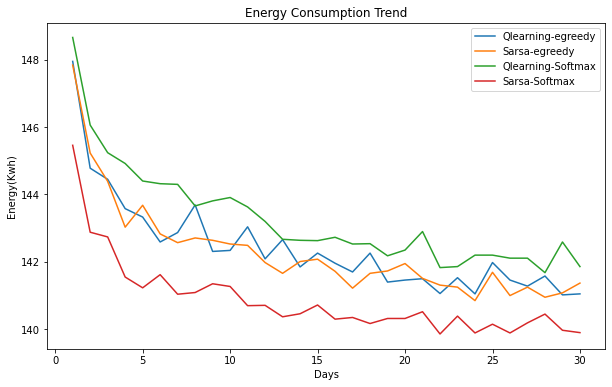
\includegraphics[width=1.0\linewidth]{Figures/Energy_Consumption_Convergence.png}
             \caption{Energy Consumption for 30 days workload}
             \label{fig:enter-label}
         \end{figure}

         \section{Total Migrations:}
          The 30 day trend for total migrations is shown belowin fig 9.2. Sarsa softmax consistently perform well in all the days compared to the other algorithms  with a standard deviation of 980.The Q learning softmax shows the worst trend compared to the others  with a standard deviation of 1230.
         
         \begin{figure}[H]
             \centering
             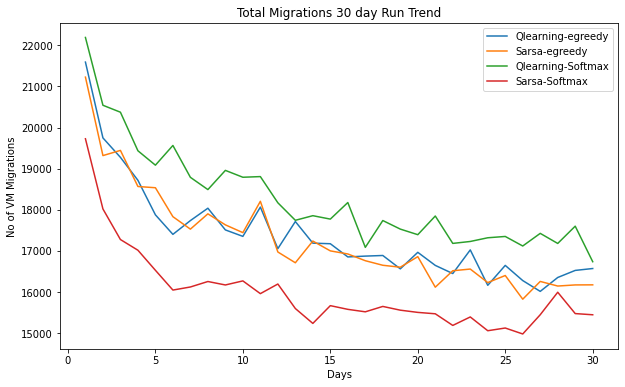
\includegraphics[width=1\linewidth]{Figures/Total_Migrations_Convergence.png}
             \caption{Total Migrations for 30 days workload}
             \label{fig:enter-label}
         \end{figure}

         \section{SLAV\%:}
          The 30 day trend for SLAV\%  is shown in fig 9.3 Again, Sarsa softmax consistently delivers  better SLA compared to the other algorithms  with a standard deviation of 0.00025\%. The sarsa $\epsilon$ greedy  shows least improvement compared to the others  with a standard deviation of 0.0032\% , followed by Qlearning softmax at 0.00028\% and Qlearning $\epsilon$ greedy at 0.00027\%
         
         \begin{figure}[H]
             \centering
             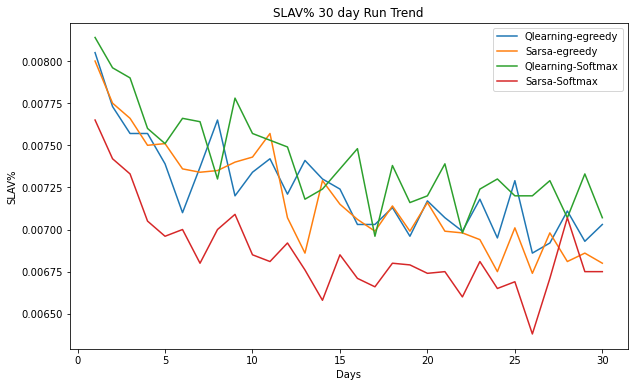
\includegraphics[width=1\linewidth]{Figures/SLAV_30day_Convergence.png}
             \caption{SLAV for 30 days workload}
             \label{fig:enter-label}
         \end{figure}

         \section{ESV:}
         The 30 day trend for ESV  is shown in fig 9.4. Sarsa softmax consistently delivers  better SLA compared to the other algorithms  with a standard deviation of 0.00044. The Sarsa $\epsilon$ greedy  shows least improvement compared to the others  with a standard deviation of 0.0055 , followed by Qlearning softmax at 0.00051 and Qlearning $\epsilon$ greedy at 0.00049.

         \begin{figure}[H]
             \centering
             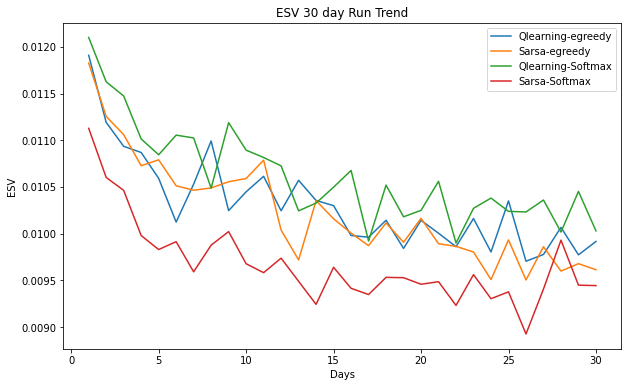
\includegraphics[width=1\linewidth]{Figures/ESV_30day_Convergence.png}
             \caption{ESV for 30 days workload}
             \label{fig:enter-label}
         \end{figure}

         \section{Conclusion:}
         From the above experiments , it can be  concluded that the Sarsa sofmax algorithm has the best performance among the four combinations we experimented.so,  For our comparison with the state of the art Lr-Mmt Algorithm , the RL algorithm Sarsa softmax will be used .Also it can be observed from the trend graphs ,the agent is able to continuously learn  with the interactions with the  Environment and  converge to an optimal value . This gives an advantage in real world where we can use the pre trained model and expect optimal operations within few interactions.
	
	\chapter{Benchmarking with Lr-Mmt}
	\label{chap:benchmarking with lrmmt}

         \section{Introduction:}
         In this chapter , the best agent from the previous experiments (ie SARSA softmax)  is compared with the benchmark algorithm - Lr-MMt .The comparison of different algorithms and the significance of  each  hyperparameters is already detailed in the previous chapter.


        \section{Standard Algorithms:}
        The research by Beloglazov is a mostly cited research in the area of VMs consolidation with respect to data center energy efficiency.To identify if the Host is over utilized, the Local Regression Policy is suggested.This policy decides a host is likely to be over utilized, if the current CPU time is larger than maximum possible utilization.
        Beloglazov suggests three  VM selection policies : Minimum Migration Time, Maximum Correlation and Random selection Policy .\cite{calheiros2011cloudsim}
        The experiments run  with the RL based algorithm is bench marked with Minimum Migration Time.
    
        \subsection{Minimum Migration Time:}
        Minimum Migration Time(Mmt) policy selects VMS to be migrated from a host based on the lowest RAM utilization as the VM with less RAM can be easily moved with less bandwidth .The VM is selected based on the following utilization.

        \begin{equation}
        \frac{RAM(VM)}{Spare_NET_Bandwidth_host}
        \end{equation}

        \section{Experimental Setup:}
        A 30-day workload is generated by randomly selecting from the existing PlanetLab workload data. The number of hosts is consistently set at 800. The number of VMs for each day is determined by the available workload files for that day in the PlanetLab dataset.
        The experiment is conducted using two algorithms, best Agent in RL  and LrMmt. The results are explored in the following sections.

        \section{Energy Consumption:}
        The Energy consumption for  a 30 day workload for the two algorithms is shown below. It can be seen that the Energy usage with lrRL is consistently less than LrMmt  in all days. The average energy usage in Lr-RL over 30 day period  is 17\% less than that of Lrmmt over the 30 day period .This amounts to energy savings of about 766 kWh over the 30 day period. Converting to average  daily usage savings of about 25 kWh.A paired t-test shows that there is a statistically significant difference in the consumption of energy when utilising Lr-RL and Lr-Mmt resulting in a P-value <0.00169 with a 95\% confidence interval (-26.2552, -23.2073).

        \begin{figure}[H]
            \centering
            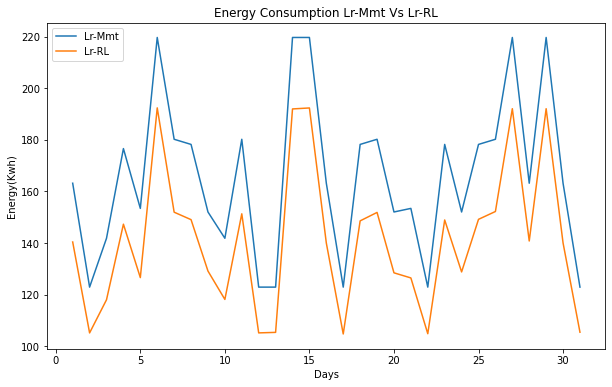
\includegraphics[width=0.75\linewidth]{Figures/Energy_Consumption_30day.png}
            \caption{Lr-RL Vs LrMmt Energy Consumption for 30 day run}
            \label{fig:enter-label}
        \end{figure}
        
        \section{Total Migrations:}
        
        The Total Migrations for  a 30 day workload for the two algorithms is shown below. Its observed that the Total VM migrations  with LrRL is consistently less than LrMmt  in all days. The average VM migrations in Lr-RL over 30 day period  is 25\% less than that of Lrmmt over the 30 day period .A paired t-test shows that there is a statistically significant difference in the total VM migrations  when utilising Lr-RL and Lr-Mmt resulting in a P-value <0.00001 with a 95\% confidence interval (-12992, -11556).

        \begin{figure}[H]
            \centering
            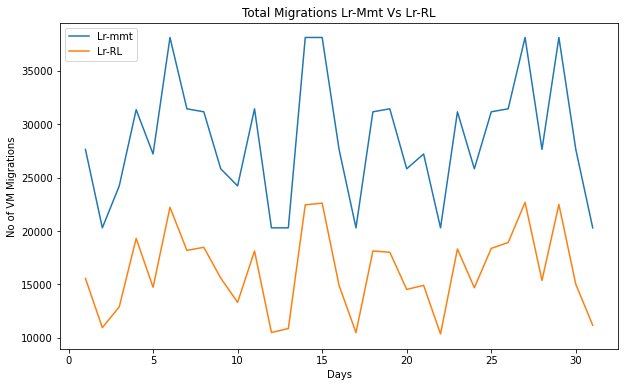
\includegraphics[width=1.0\linewidth]{Figures/Total_Migrations_30day.png}
            \caption{Lr-RL Vs LrMmt Total Migrations for 30 day run}
            \label{fig:enter-label}
        \end{figure}

        \section{SLAV:}

        The Service Level Agreement Violation percentage   for  a 30 day workload for the two algorithms is shown below. It can be seen that the SLAV percentage  with lrRL is slightly less than that of LrMmt . With the lesser Total  migrations and less energy consumption's , the LrRL is expected to show a reduced  SLAV  compared to LrMmt.A paired t-test shows that there is a statistically significant difference in the total SLAV\%  when utilising Lr-RL and Lr-Mmt resulting in a P-value <0.00001 with a 95\% confidence interval (0.00201, 0.00233).

        \begin{figure}[H]
            \centering
            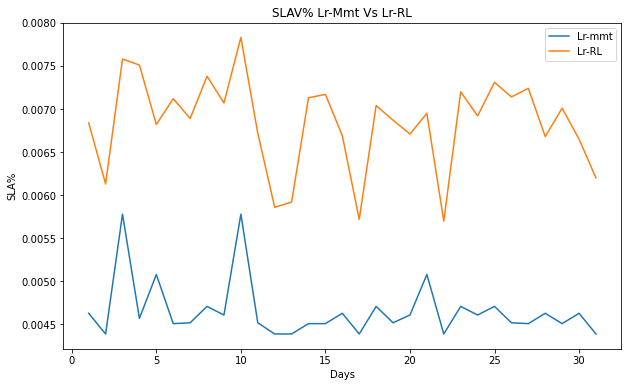
\includegraphics[width=1.0\linewidth]{Figures/SLAV_30day.png}
            \caption{Lr-RL Vs LrMmt SLAV\% for 30 day run}
            \label{fig:enter-label}
        \end{figure}

        \section{ESV:}
        ESV is an important metric that comprises both the SLAv and the Energy Consumption. LrRL under performs when compared to the LrMmt.
        A paired t-test shows that there is a statistically significant difference in the total SLAV\%  when utilising Lr-RL and Lr-Mmt resulting in a P-value <0.0001 with a 95\% confidence interval (0.0016, 0.0023).

        \begin{figure}[H]
            \centering
            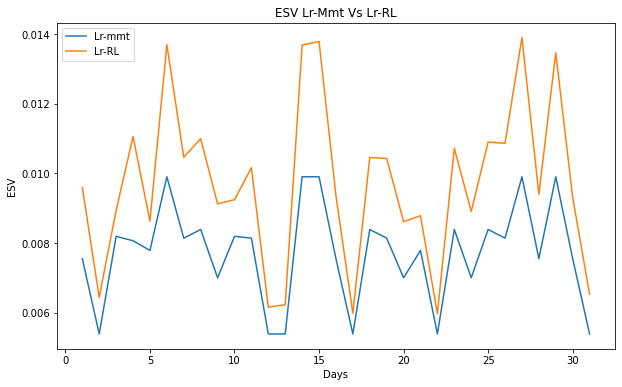
\includegraphics[width=1.0\linewidth]{Figures/ESV_30day.png}
            \caption{Lr-RL Vs LrMmt ESV for 30 day run}
            \label{fig:enter-label}
        \end{figure}
        

	\section{Conclusion:}
         The Lr-RL algorithm is able to reduce the Energy Consumption and the total migrations over the standard benchmarking algorithm LrMmt . Reducing the number of VM migrations helps to reduce the Energy Consumption. However this doesn't proportionally translate to the SLAV or ESV . The SLAV and ESV performs poorly than the LrMmt algorithm . This area requires further study and optimization in future work.

	\chapter{Summary}
	\label{chap:Summary}
         In this thesis, a series of experiments were conducted utilizing the Lr-RL algorithm, which were then benchmarked against the industry standard, Lr-Mmt algorithm. Initially, two reinforcement learning algorithms, Q-learning and SARSA, were analyzed. Subsequent experiments employed two distinct policies—epsilon-greedy and SoftMax—to determine the most effective hyperparameters, specifically the learning rate (alpha) and the discount factor (gamma)
         
        In the 30-day workload analysis(chapter 8), it was observed that a higher learning rate significantly improves energy consumption values when using the Q-learning algorithm. Conversely, for the SoftMax policy, energy consumption values remained relatively stable, showing minimal sensitivity to variations in the learning rate (gamma).

        A higher learning rate $\alpha$ means that the agent gives more weight to new information and updates its Q-values more aggressively after each action. This allows the agent to learn faster, especially in dynamic environments where conditions may change frequently.While a higher learning rate can speed up learning, it can also make the learning process less stable. The agent might overreact to recent experiences, leading to oscillations or instability in the Q-values. This can result in a less optimal policy if the environment is noisy or if the learning rate is too high. A lower discount factor $\gamma$ indicates that the agent prioritizes immediate rewards over future rewards. This can be useful in environments where future rewards are uncertain or less reliable. The agent becomes more focused on achieving immediate gains rather than considering long-term outcomes.Consequently, the most effective algorithm and its optimal hyperparameters were selected based on these findings.
        
        In chapter 10, the LrRL algorithm is benchmarked against the LrMmt, with respect to the  metrics such as energy consumption, total VM migrations, service level violations, and ESV. These metrics are systematically tabulated to evaluate the performance of the LrRL in comparison to LrMmt. The analysis reveals that LrRL significantly reduces both energy consumption and the number of VM migrations. These findings address the \textit{first research question} of the thesis, confirming that reducing the number of VM migrations can indeed enhance the energy efficiency of the data center.
        
        However, this effect is not mirrored in the other two parameters: SLAV (Service Level Agreement Violations) and ESV (Energy Savings Value). This observation addresses the \textit{second research question}, which probes whether SLAV percentage is proportional to the total number of VM migrations. The findings suggest that additional external factors, such as host bandwidth, may need to be considered during VM migrations. The RL algorithm, in its pursuit of minimizing VM migrations, tends to select the largest VM in the overloaded host. Unfortunately, the data collected does not support the effectiveness of this aggressive strategy. Consequently, there is a need to reformulate the reward function to incorporate other critical factors such as available bandwidth.
        
        Chapter 9  addresses the \textit{third research question} whether the reinforcement learning (RL) algorithm improves its performance through successive interactions—a single workload was replicated 30 times, simulating a 30-day period Observations from this experiment reveal a decreasing trend in energy consumption, indicating that the agent is learning and optimizing its decisions over time. This trend supports the hypothesis that the RL algorithm effectively adapts and enhances its performance through repeated interactions with the environment.

        
	%%%%%%%%%%%%%%%%%%%%%%%%%%%%%%%%%%%%%%%%%%%%%%%%%%%%%%%%%%%%%%%%%%%%%%%%%%%%%%%%
	%\bibliographystyle{plainnat}                  % to give author-year style
	\bibliographystyle{IEEEtranN} 
	\renewcommand{\bibname}{References}           % change default name Bibliography to References
	\bibliography{references}                     % BibTeX References file, references.bib
	\addcontentsline{toc}{chapter}{References}    % add References to TOC
	
	
	%%% uncomment if Appendix needed
	\appendix
	\chapter{Code} 
	\label{chap:appendix_a}

         
         \section{Description:}
         The complete code for the project is available in the   \href{https://github.com/mniju/Masters_Thesis}{github repository} 

         Link: https://github.com/mniju/Masters\_Thesis
    
         \noindent The Lr-RL implementation is implemented with the codebase  \href{https://github.com/Cloudslab/cloudsim/releases/tag/cloudsim-3.0.3}{cloudsim-3.0.3}
         
	%\chapter{Appendix-B-Title} 
	%\label{chap:appendix_b}
	
\end{document}
